\label{chap-gds}

\section{Introduction}
\label{gds-intro}

In the previous chapter multidimensional scaling was used to project the points within some geographical area into a new space in which smoothing can be performed without the problem of leakage. However, it has become clear that there is a trade-off involved in using this method: if the ordering of the points in space is to be maintained (\secref{pensuck}), a sufficiently high dimensional projection of the data must be obtained. Increasing the projection dimension causes the nullspace of the thin plate spline penalty (\secref{GAMtprspenalty}) to become large, causing a large space of wiggly functions to be used without being penalised, leading to unreliable smoothing results (\secref{nohigherdim}). To resolve this issue, a smoother which can deal with high dimensional data must be used. 

High dimensional smoothing has been approached in several different ways previously, these include:
\begin{enumerate}
   \item Without straying too far from thin plate splines, one could consider using tensor products of splines of any basis (\secref{GAMtensor}). For example, marginal smooths of P-splines (\secref{intro-psplines}) could be combined using a tensor product to create a multidimensional smooth in the requisite number of dimensions. In practice several problems arise with this approach. First is the problem of knot placement, which in high dimensions can become massive computational burden, requiring some kind of knot selection. Second is that tensor product smooths are anisotropic so one smoothing parameter is used per dimension, aside from the additional computational burden, the point of the high dimensional projections used is in part to combat anisotropy. Finally, although the marginal functions in a tensor product smooth can be simple, the combination of the functions can turn out to require many evaluations.
   \item Rather than using a basis function decomposition of the smoother, local regression could be used. Two popular local regression techniques are LOESS which smooths the data using a low-degree local polynomial  (\cite{loess1}, \cite{loess2}) or kernel smoothing by taking weighted averages of the response with weightings based on distance (e.g. \cite[pp. 194-200]{elements}). Local methods are, of course, local and as such rely on the data being relatively dense, which cannot be guaranteed, especially in high dimensions (\cite[p. 200]{elements}). 

Integrating these methods into a GAM (which is desirable so that other terms and other smoothers can be included in the model) requires backfitting be used for the fitting prodecure. Backfitting consists of smoothing the residuals with respect to that component's covariate. However, backfitting is quite computationally expensive since smoothing parameters must be selected at every stage (i.e. each time a set of residuals is smoothed).

   \item Kriging could be used to smooth in high dimensions, however there are technical limitations on the number of dimensions that are possible. In particular ensuring that the semivariogram remains positive definite (\cite{boisvert}). Although there has been work using MDS to obtain isotropic distances for semivariogram estimation, there has not been work on how to deal with the mean field when it is non-constant, incorporating a trend into the mean field when it has been projected into high dimensions will lead to similar difficulties as in the spline smoothing case. This is covered in more detail in \secref{gds-krig}.
\end{enumerate}

All of the methods listed above have problems that thin plate splines do not suffer from. Thin plate splines do have the problem that the number of functions in nullspace of the penalty becomes far too large when smoothing is performed in high dimensions (see figure \ref{nullspace-dim}). Limiting the number of functions in the nullspace of the penalty would avoid the side effects of having complicated, unpenalised functions in the resulting smooths. 

When originally proposing thin plate splines in his seminal 1977 paper, Duchon actually describes a much more general set of interpolation methods; thin plate splines are just a particular example of these. This chapter illustrates how a more general version of the thin plate spline (henceforth referred to as Duchon splines) can be used for high dimensional smoothing whilst avoiding a large and complex penalty nullspace.

The next section goes into the technical detail of how Duchon splines work and how they can be used in the finite area smoothing case. \Secref{gds-wad-examples} shows how this can be useful in the within-area distance case discussed in chapters \ref{chap-sc} and \ref{chap-mds}. \Secref{gds-gds-examples} expands the methodology to look at any problems where distances can be considered, taking the MDS projection of these distances and then smoothing in the projected space. \Secref{gds-software} illustrates the software implementation of these methods. \Secref{gds-krig} compares the methods developed here with similar methods used in kriging. Finally, \secref{gds-conclusion} concludes the chapter.

\section{Using Duchon splines for reliable high dimensional smoothing}

This section starts from the definition of the thin plate spline penalty and shows how one can motivate the more general Duchon spline penalty. The aim is to show how the penalty works and that the main differences between it and the thin plate spline. A full technical exposition (from a mathematical rather than statistical point of view) is given in \citeb{duchon77}. This section goes on to show how (once reliable high dimensional smoothing can be performed) the size of the MDS projection dimension can be selected.

\subsection{From thin plate splines to Duchon splines}
\label{gds-tprstoduchon}

First re-iterating and expanding on the description of thin plate splines given in the introduction, the thin plate spline penalty (as given in (\ref{tprs-pen})) in $d$ dimensions with derivative order $m$ is :
\begin{equation*}
J_{m,d} = \int \ldots \int_{\mathbb{R}^d} \sum_{\nu_1 + \dots + \nu_d=m} \frac{m!}{\nu_1! \dots \nu_d!} \left( \frac{\partial^m f \left (x_1,\dots,x_d \right )}{\partial x_1^{\nu_1} \ldots  \partial x_d^{\nu_d}} \right)^2 \text{d} x_1 \ldots  \text{d} x_d,
\end{equation*}
where the summation index generates all of the possible combinations of derivative orders such than their sum is still $m$ (thereby finding all the correct cross-terms for the derivatives). In order to ensure that $f$ remains continuous, $2m>d$.

It can then be shown that the thin plate spline basis minimizes (\ref{tprs-pen}) and is given by:
\begin{equation*}
f(\mathbf{x}) = \sum_{i=1}^n \delta_i \eta_{md}(\mathbf{x}-\mathbf{x_i}) + \sum_{j=1}^M \alpha_j \phi_j(\mathbf{x}),
\end{equation*}
where the first summation is a set of radial basis functions ($i$ indexing the $n$ data) and the second summation are a set of (global) linearly independent polynomials of degree less than $m$. The terms in the second summation are unpenalised (since their derivatives are zero).  There are $M$ of these polynomials lying in the nullspace of the penalty, where $M$ is given by:
\begin{equation}
M=\begin{pmatrix} m+d-1 \\ d  \end{pmatrix}.
\label{gds-bigm}
\end{equation}
In the cases presented so far, $d$ (the MDS projection dimension) is known and $m$ is dictated by $d$, since $2m>d$. $M$ therefore increases very quickly with the number of dimensions; this is shown by the blue line in figure \ref{nullspace-dim}. As more basis functions are included in the nullspace, the more complex the functions are. A large number of increasing complex, global functions which are unpenalized pose a serious threat to the fitting of parsimonious models.

\begin{figure}
\centering
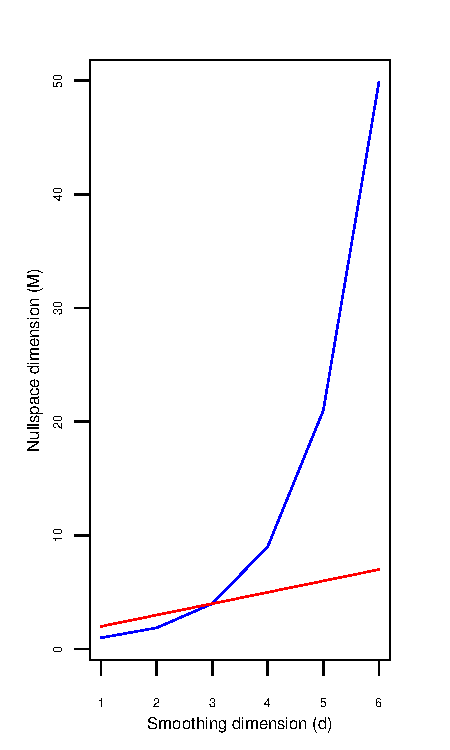
\includegraphics[width=3in]{gds/figs/nullspace-dim.pdf} \\
\caption{Relationship between smoothing dimension ($d$) and the nullspace dimension ($M$) when $m$ (the derivative penalty order) is set to 2 for thin plate regression splines (blue) and Duchon splines (red). Note that as the nullspace dimension increases, the complexity of those functions in the nullspace increases too. For the thin plate splines a combination of the continuity condition that $2m>d$ and the form of $M$ (see (\ref{gds-bigm})) makes the size of the nullspace increase very quickly with smoothing dimension.}
\label{nullspace-dim}
% generated by thesis/mds/figs/nullspace-dim.R
\end{figure}

Starting from (\ref{tprs-pen}), the first step toward the more general Duchon penalty is to consider taking the Fourier transform of the derivatives before squaring and integrating them. The Fourier transform allows us to consider the penalty as an infinite sum of frequencies; decomposing functions defined in space into their frequency domain representations. Mathematically, the Fourier transform $g$ a function $\mathbf{x}$ (a $d$-vector), is defined as:
\begin{equation*}
\mathfrak{F} g(\boldsymbol{\tau}) = \int \ldots \int_{\mathbb{R}^d} e^{2 \pi \sqrt{-1} \mathbf{x}^\text{T} \boldsymbol{\tau}} g(\mathbf{x}) \text{d}\mathbf{x}.
\end{equation*}
Here $\mathfrak{F}$ is an operator applied to $g$, so $\mathfrak{F}g$ may be considered as a function of $\boldsymbol{\tau}$ (a $d$-vector of continuous frequencies). More detail on Fourier transforms can be found in \citeb{bracewell}, \citeb{chu-ft} and \citeb{beerends}. 

Taking the Fourier transform of the penalty allows us to think of how the penalty is calculated in a different way. Rather than thinking about measuring the wigglyness of each basis function, the penalty is calculated from measuring the intensity of the different frequencies of $f$ over the whole domain, weighted so that higher frequency components contribute more to the integral than the lower ones. Intuitively, the low frequency components of the derivatives of $f$ are likely performing a similar task to those functions in the nullspace of the penalty, where as the more complicated, high frequency components are more complicated parts of the function, likely to be the parts of $f$ that attempt to interpolate the data.

Taking the Fourier transform of the derivative terms in (\ref{tprs-pen}) yields the following penalty:
\begin{equation}
J_{m,d} = \int \ldots \int_{\mathbb{R}^d} \sum_{\nu_1 + \dots + \nu_d=m} \frac{m!}{\nu_1! \dots \nu_d!} \left ( \mathfrak{F} \frac{\partial^m f}{\partial x_1^{\nu_1} \ldots  \partial x_d^{\nu_d}} \left (  \boldsymbol{\tau}\right ) \right )^2 \text{d} \boldsymbol{\tau}.
\label{tprs-pen-ft}
\end{equation}
The penalties (\ref{tprs-pen}) and (\ref{tprs-pen-ft}) are in fact equivalent by Plancherel's theorem (\cite{vretblad}, p. 180) in the sense that they evaluate to the same numerical value.

Since taking the Fourier transform of the derivatives has allowed us to think of the derivatives as made up of frequencies, it then follows to exploit this interpretation by introducing a weighting into the penalty: 
\begin{equation}
\int \ldots \int_{\mathbb{R}^d} w(\boldsymbol{\tau}) \sum_{\nu_1 + \dots + \nu_d=m} \frac{m!}{\nu_1! \dots \nu_d!} \left ( \mathfrak{F} \frac{\partial^m f}{\partial x_1^{\nu_1} \ldots  \partial x_d^{\nu_d}} \left (\boldsymbol{\tau} \right ) \right )^2 \text{d} \boldsymbol{\tau},
\label{duchon-penalty-general}
\end{equation}
the function $w$ can then be used to pick out particularly high frequencies and penalise those more than the lower frequency ones. Setting $w(\boldsymbol{\tau})=1, \forall \boldsymbol{\tau}$ allows us to recover (\ref{tprs-pen}).

Duchon suggests the use of $w(\boldsymbol{\tau})= \lvert \boldsymbol{\tau} \rvert^{2s}$. This will still give a minimizer of broadly the same form as the thin plate spline functions in (\ref{tprs-basis}) but $M$ will change. First writing down this penalty:
\begin{equation}
\breve{J}_{m,d} = \int \ldots \int_{\mathbb{R}^d} \lvert \boldsymbol{\tau} \rvert^{2s} \sum_{\nu_1 + \dots + \nu_d=m} \frac{m!}{\nu_1! \dots \nu_d!}\left ( \mathfrak{F} \frac{\partial^m f}{\partial x_1^{\nu_1} \ldots  \partial x_d^{\nu_d}} \left (\boldsymbol{\tau} \right ) \right )^2 \text{d} \boldsymbol{\tau}.
\label{duchon-penalty}
\end{equation}
The less complex (more smooth) frequency components of the basis functions are penalized less. This allows some of the fequencies of  the radial basis functions to do the job of the polynomials which were not included due to reduced nullspace size. The penalty allows the use of a reduced nullspace (in both size and complexity terms) while not sacrificing the continuity of $f$. 

Again, (\ref{tprs-pen}) can be recovered from this penalty (by setting $s=0$). When $s>0$ higher frequencies are penalised more than lower ones. In order to obtain smooth functions it is required that $m+s>d/2$ (this replaces the condition that $2m>d$ for thin plate splines). So $s$ can be used to allow high dimensional smoothing, while still using lower-order penalties without yielding discontinuous functions. One can therefore think of $s$ as a kind of ``fudge factor'' that allows the conditions on $m$ and $d$ to be relaxed. Given some fixed combination of $m$ and $d$, an $s$ can be found by simply calculating:
\begin{equation}
s>d/2-m.
\label{duchon-s-eqn}
\end{equation}
For the examples below, the smallest integer $s$ is used with $m=2$, so:
\begin{equation}
s=d/2-1.
\label{duchon-s-eqn2}
\end{equation}

The red line in figure \ref{nullspace-dim} gives the number of functions that lie in the nullspace of penalty (\ref{duchon-penalty}), i.e. the result of using (\ref{duchon-s-eqn2}) with (\ref{gds-bigm}). For plotting $m=2$ so the derivative order is constant as the dimensionality increases, leading to a linear increase in nullspace size with the smoothing dimension.

%[[\textbf{SIMON} : If I can construct some kind of proof that the MDS projection of within-area distances always leads to a manifold then I'll say something here about how that leads to the following \ldots In any small region a 2-dimensional manifold will look like $\mathbb{R}^2$, in the same small region the smoother's behaviour will closely approximate a regular thin plate regression spline with $m=2$ on the tangent space of the manifold (as the smoothing parameter tends to zero, at least).]]

These splines have been largely neglected in statistical smoothing literature with the exception of \citeb{girosi} which discusses the connections between neural networks and GAMs with the more general form of this type of penalty (ie. (\ref{duchon-penalty-general})). \citeb[p. 168]{elements} also discuss Girosi's work briefly.

\subsection{Duchon splines with \mdsap\ -- \mdsds}

With the addition of Duchon splines to the \mdsap\ we are now in a position to project data into higher dimensions and smooth over the response without having to worry about the the size and complexity of the nullspace causing problems. The use of Duchon splines along with \mdsap\ and the projection dimension selection techniques below will be known as \mdsds\ (Multidimensional Scaling for GAMs) from here on.

\subsection{Choosing MDS projection dimension}

With Duchon's basis, it is now possible to smooth over any number of dimensions whilst using second order derivatives in the penalty, simply by picking $s$ according to (\ref{duchon-s-eqn}). For the within-area distance cases considered here, the resulting MDS configurations look like 2-dimensional manifolds. Indeed, it is reasonable to assume that the projection space will look like a 2-dimensional manifold at least locally since near every point the neighbouring points will be mostly Euclidean rather than within-area distances. 

Picking the dimension of the MDS projection is now a concern since there is no reason to believe that simply going to higher and higher dimensions will yield better results. For reasons of model parsimony, it is preferable to use as low a projection dimension as possible.

\subsubsection{Using the spectral norm}

As discussed in \secref{nohigherdim}, as higher dimensional projections are used, a larger and larger proportion of the variation in the distance matrix is explained. It therefore seems reasonable to base the choice of dimension on the proportion of the variation explained in the initial grid. However, what proportion should be used? 80\%? 90\%? 99\%? There is no reason \textit{a priori} to choose any one of these over the others. Setting the proportion of variation to be explained without thought of the domain in question is surely a bad idea, since what works for one domain may well be a disaster for another. Such an approach also does not take into account the response values, thus discarding useful information.

\subsubsection{Using scores}

Since fitting a smooth of Duchon splines and using MDS to project the distance matrix is relatively cheap compared to the cost of finding the within-area distances, it is not problematic to fit many models (varying the projection dimension) provided no new distances need to be calculated. 

For this reason the GCV score can be used to find an optimal dimension for the MDS projection. A series of (increasing dimensional) projections can be tried, their GCV scores calculated, and the best selected as the projection to use for the model. As mentioned above, the GCV score also takes into account model fit rather than just variation.

Starting from a 2-dimensional projection, the dimensionality is increased and models fitted. The upper bound is the number of dimensions that explain 95\% (say) of the variation in the distance matrix of the initial grid (see section \ref{grids}). Although a complete search on all dimensions could be performed, this could become extremely time consuming and it is likely that higher dimensions offer very little difference in the point configuration given that the associated eigenvalues will become smaller and smaller. It is also possible to proceed step-wise and stop once the GCV score starts to increase, however there is no good reason to believe that the GCV score would be unimodal in the number of dimensions. Looking at plots such as those in figure \ref{wt2-gcv-projdim-boxplot} gives guidance on how to proceed. Throughout the following analyses all dimensions between 2 and that which explains 95\% of the variation in the distances are tested.

Simulations show that the minima in the GCV score and MSE are in agreement. For example figure \ref{wt2-gcv-projdim-boxplot} shows a plot of GCV score and mean squared error for 60 simulations from the peninsula domain, for each of the 60 realisations \mdsds\ was fitted using a 2 through 20 dimensional projection. The boxplots are grouped according to the dimension of the MDS projection used. The graph shows that there is a minima in the score when the dimension is four, this corresponds with the minimum MSE.

\begin{figure}
\centering
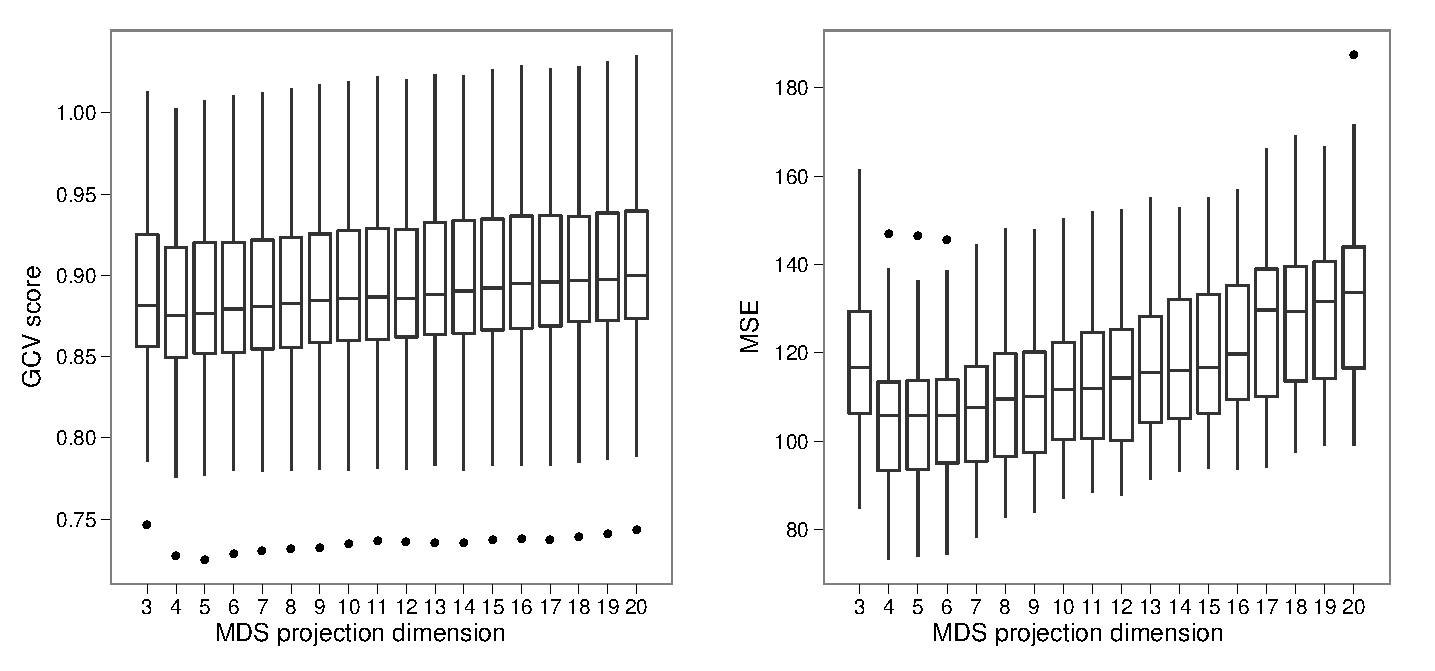
\includegraphics[width=6in]{mds/figs/wt2-gcv-projdim-boxplot.pdf} \\
\caption{MSE and GCV score for the peninsula domain when different dimensional projections are used. Here a 4-dimensional projection minimizes both the GCV score and the MSE in simulation.}
\label{wt2-gcv-projdim-boxplot}
% generated by mds/duchon/wt2-gcvml.R
\end{figure}

If smoothing parameter selection is to be performed via ML (\secref{intro-extending-gams}), the ML score can be adapted into an AIC-like score to be used in place of the GCV score, provided there is appropriate penalisation to take into account the increase in the dimension of the projection space. Note that the REML score cannot be used as REML scores cannot be compared when fixed effects are changed (\cite{remlpaper}). The (AIC-like) score (denoted $\text{ML}_P$) used was:
\begin{equation*}
\text{ML}_P = -2 \hat{l} + 2P
\end{equation*}
where $\hat{l}$ is the log-likelihood at the MLE and $P$ is a penalty. Setting the penalty to be the nullspace dimension (i.e. $M$ from above with $m=2$ and $d$ the MDS projection dimension):
\begin{align*}
P =& \begin{pmatrix} 2+d-1 \\ d  \end{pmatrix},\\
=& \begin{pmatrix} d+1 \\ d  \end{pmatrix},\\
=& d+1.
\end{align*}
So the score used to select dimension is:
\begin{equation*}
\text{ML}_P = -2 \hat{l} + 2(d+1)
\end{equation*}

The extra penalty can be justified in the following way: it is possible that an increase in dimension (which adds much more complexity into the model) will give only a slight increase in the likelihood. This model would be taken as ``best'' even though it only offers a small improvement on a much simpler model. To avoid these models being selected, the penalty above is added.

There is, of course, no guarantee that there will always be a clear minimum to find or even that either score will be unimodal in projection dimension. As with all automated methods, diagnostics (for example the plots of score against dimension) should be used.

\section{Within-area distance examples}
\label{gds-wad-examples}
\subsection{Simulations}

To test the utility of \mdsds, the simulation study on the peninsulae domain in section \ref{wt2bigsim} was re-run including \mdsds\ as a possible model, MDS dimension selection based on both GCV and $\text{ML}_P$ scores was used and the maximum spline basis dimension was set at 100. The results are shown for the original simulations (for thin plate splines and the soap film smoother) along side those for the new model in figure \ref{wt2-boxplot-duchon}. \mdsds\ with GCV dimension selection obtained a lower MSE than the soap film smoother when the noise is low and was indistinguishable (via a paired Wilcoxon signed rank test) from the soap film smoother at higher noise levels. Using $\text{ML}_P$ generally had poorer performance but this only became significant at the highest noise level.

Using GCV does give a lower MSE than using the soap film smoother. This is a good indication that using GCV to control the MDS projection dimension is working well. Visual inspection of the smooths produced also show that the GCV score works well as a way of selecting the number of dimensions to project into.

\begin{figure}
\centering
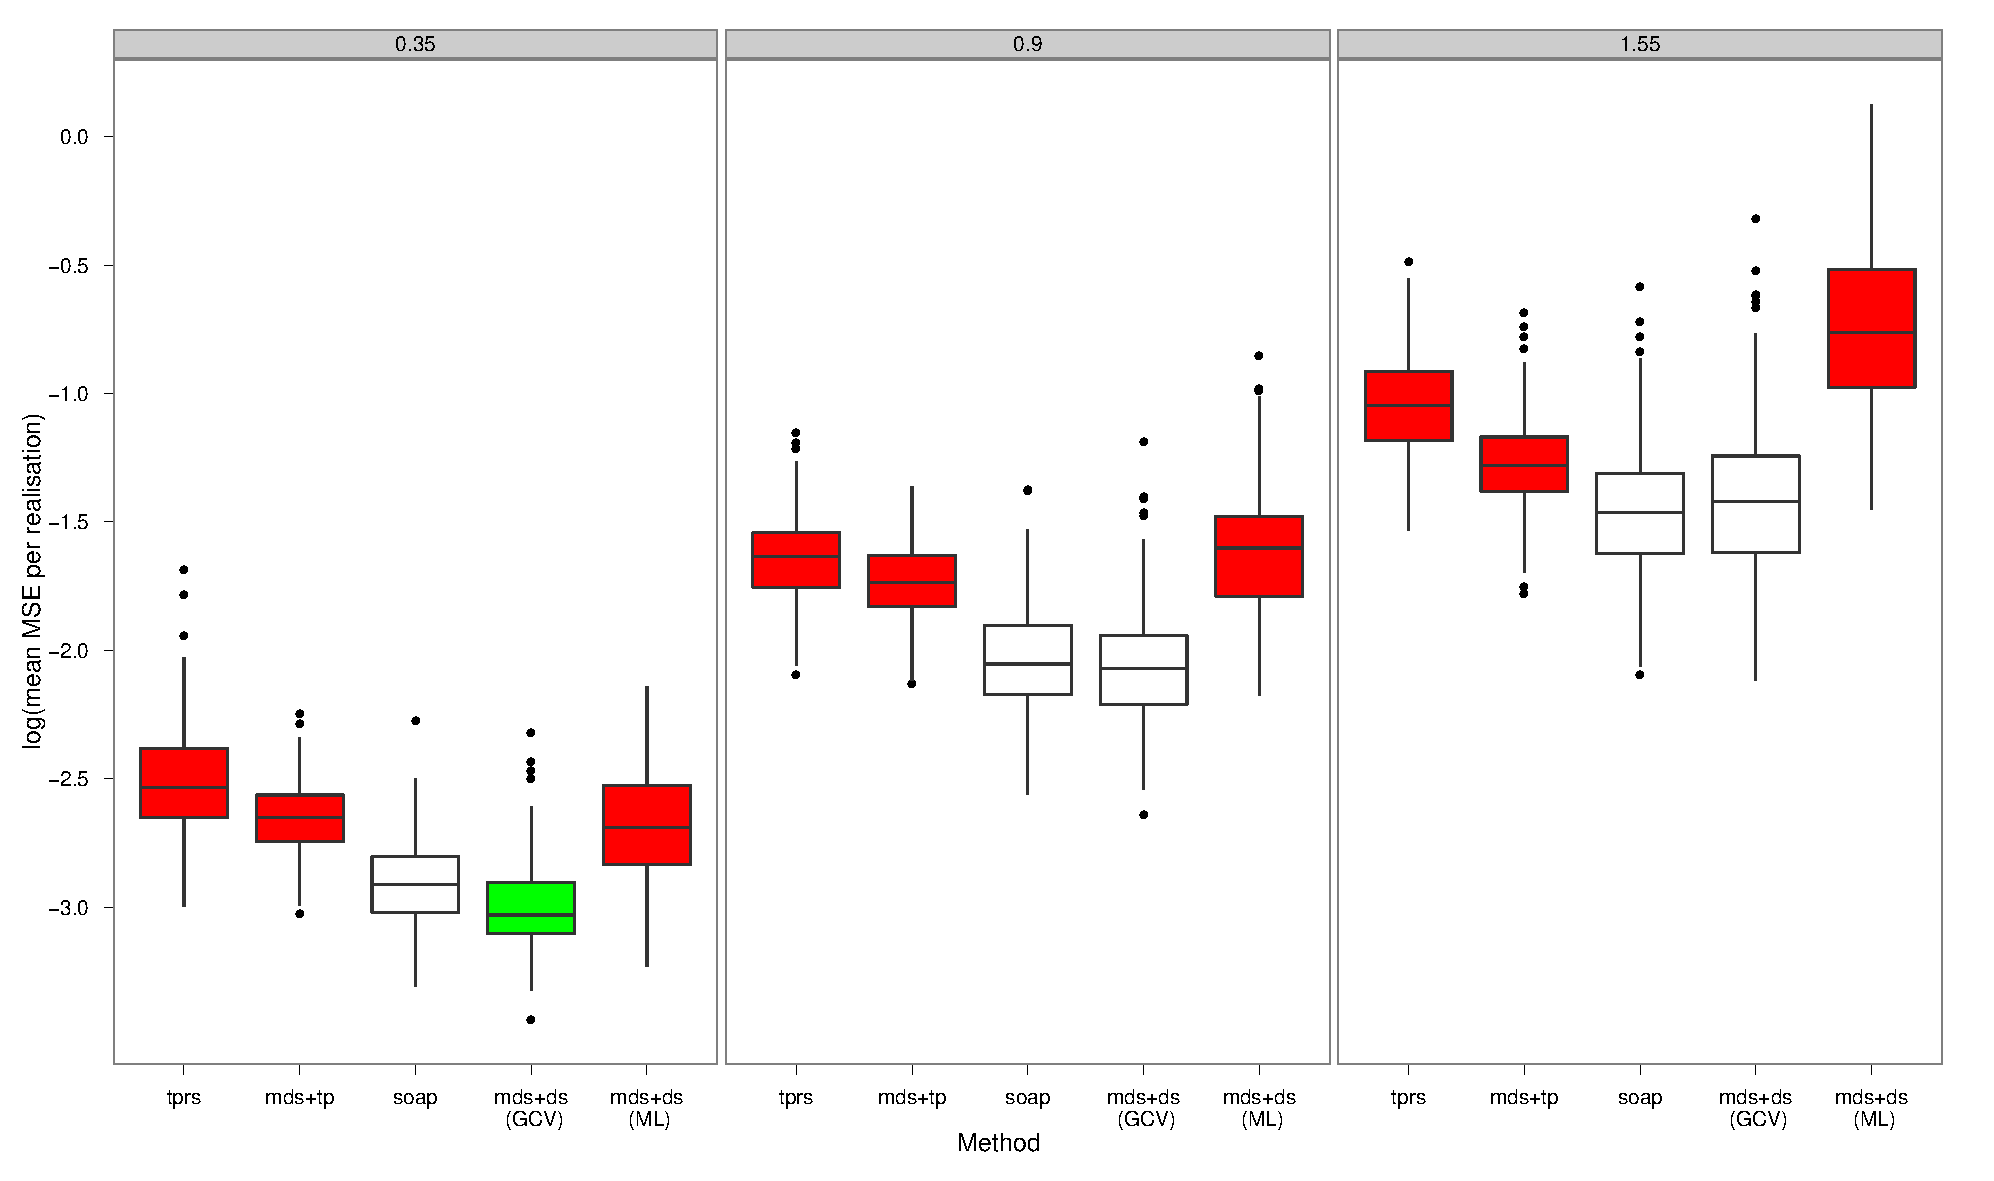
\includegraphics[width=6in]{mds/figs/wt2-boxplot-duchon.pdf} \\
\caption{Boxplots of logarithm of per realisation average mean squared error from simulations on the peninsula domain. The boxplots are in groups of four for each error level (0.35, 0.9, 1.55). Colours indicate the result of a Wilcoxon paired signed rank test of whether the MSE was significantly ($p<10^{-2}$) different from the soap film smoother. Red indicates different and worse, green different and better.}
\label{wt2-boxplot-duchon}
% generated by mds/duchon/bigsim/boxplot-wt2.R
\end{figure}


\subsection{Revisiting the Aral sea}
\label{aral-revisit}
Returning to the Aral sea example from section \ref{aral-sec}, \mdsds\ can be used to fit a model using the optimal dimension (in GCV/$\text{ML}_P$ terms). Figure \ref{mds-aral-5d-duchon} shows the raw data and a smoothed version, using a 5-dimensional projection (given by minimising the GCV score). The plot does not contain any of the artefacts that were present in the previous smooths of the data in high dimensions.

\begin{figure}
\centering
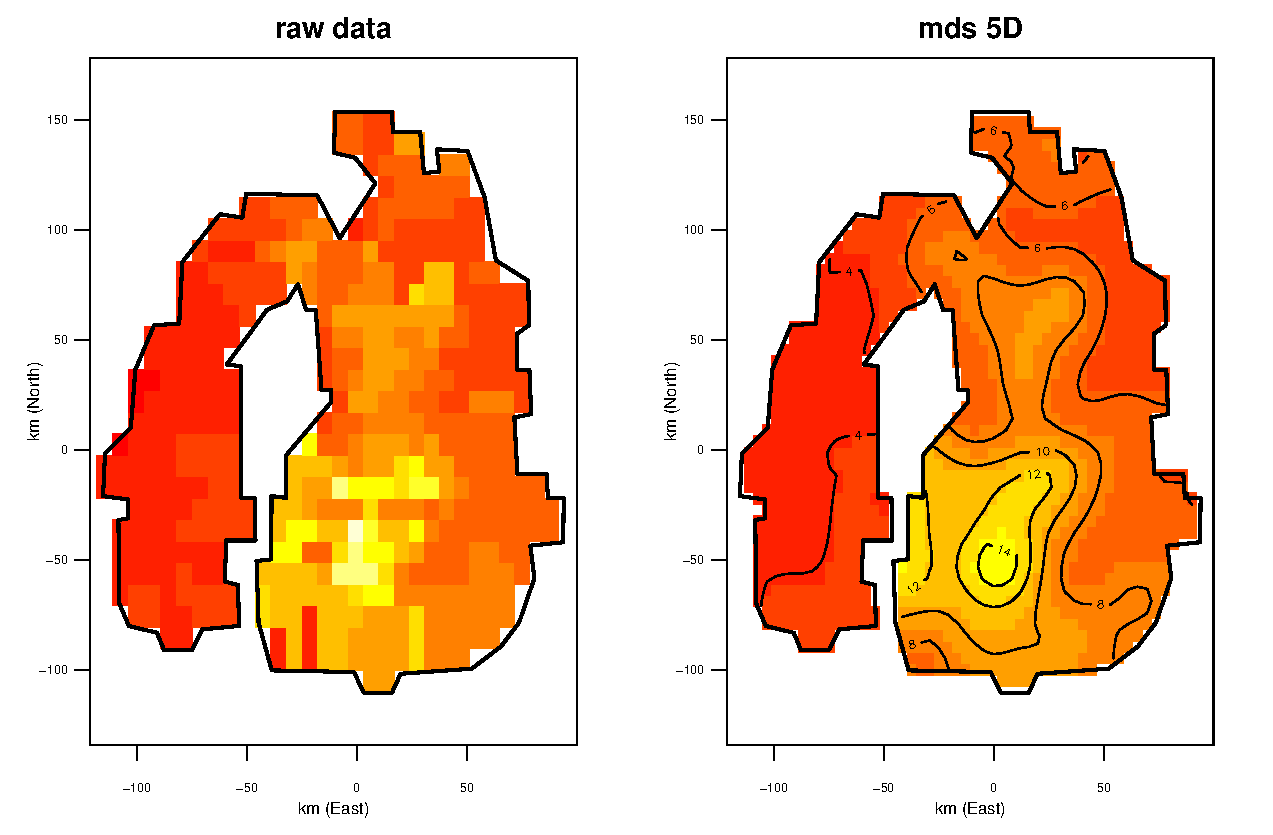
\includegraphics[width=6in]{mds/figs/aral-5d-duchon.pdf} \\
\caption{The Aral sea chlorophyl levels smoothed using \mdsds, when a 5-dimensional MDS projection is employed. Note the lack of artefacts in comparison to previous \mdsap\ models.}
\label{mds-aral-5d-duchon}
% generated by duchon/aral-evolve.R
\end{figure}

Using the $\text{ML}_P$ statistic to select the MDS projection dimension resulted in a 19-dimensional smooth, significantly greater than the dimension selected by GCV. The image plot in figure \ref{gds-aral-19d} does not look particularly different from the GCV selected one in figure \ref{mds-aral-5d-duchon}, although perhaps there is some overfitting (for example in the $(-50,100)$ and $(80,-20)$ areas). Figure \ref{gds-aral-dim-select} shows plots of score (both GCV and $\text{ML}_P$) against MDS projection dimension. The GCV plot shows a clear minima where as $\text{ML}_P$ does not. Given this plot and the marginally worse performance in the peninsulae domain simulations, it doesn't seem like $\text{ML}_P$ is a particularly good choice for projection dimension selection when using within-area distances.

\begin{figure}
\centering
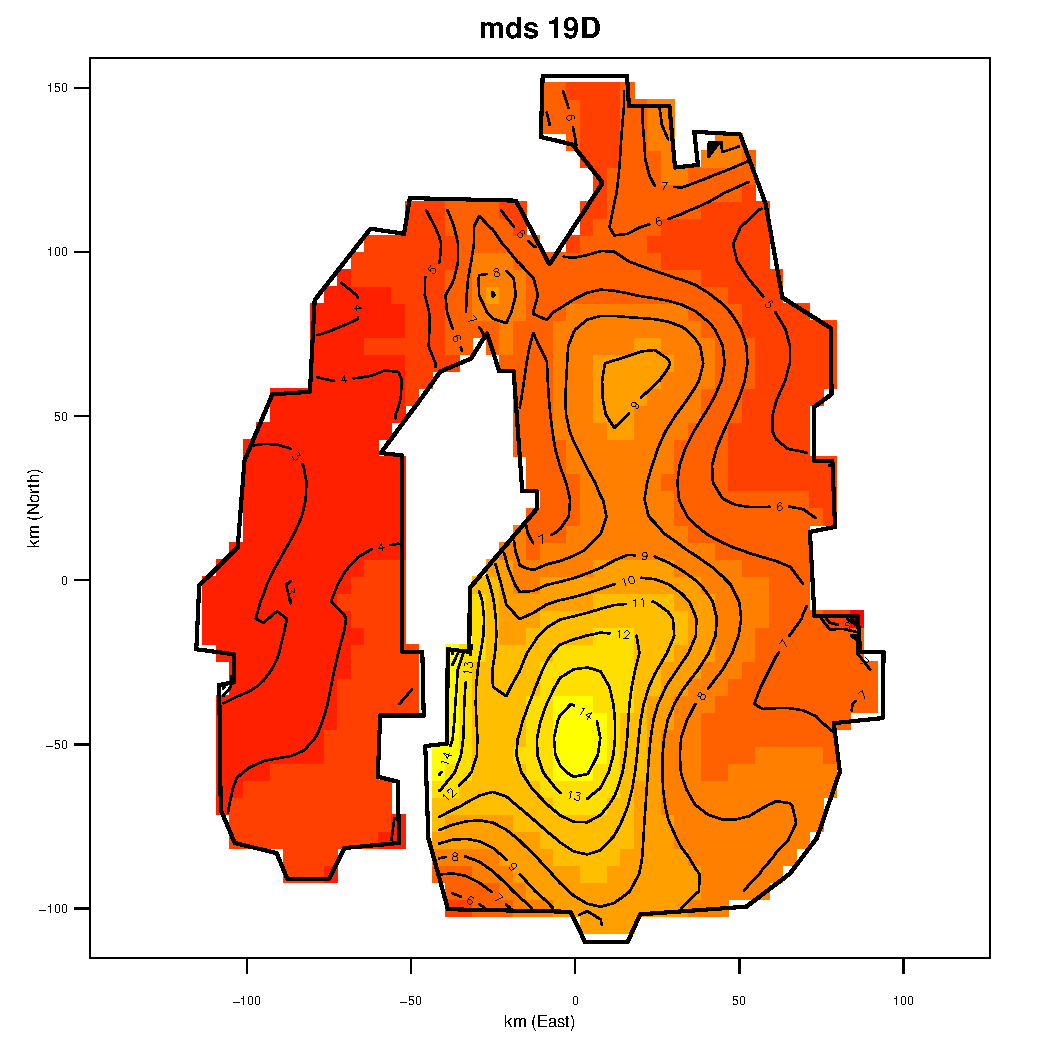
\includegraphics[width=4in]{gds/figs/aral-19d.pdf} \\
\caption{Image plot of the smoothed surface fitted by \mdsds\ for the Aral sea when $\text{ML}_P$ is used to select the MDS projection dimension.}
\label{gds-aral-19d}
% generated by duchon/aral-scoreplots.R with liberal use of commenting
\end{figure}

\begin{figure}
\centering
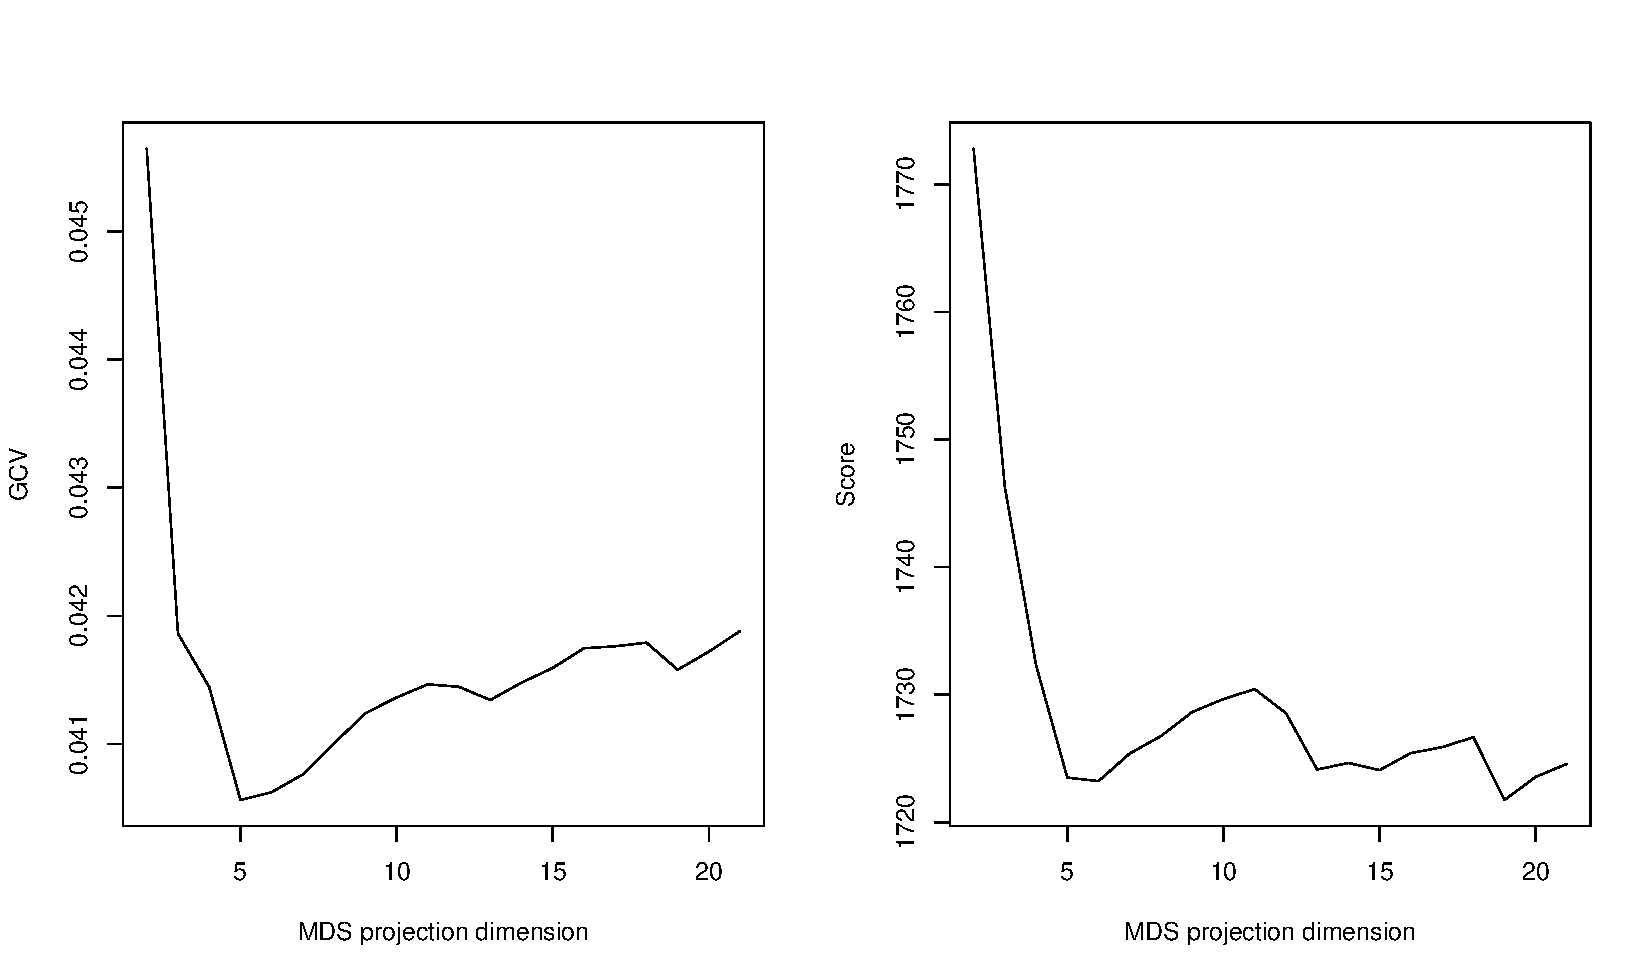
\includegraphics[width=6in]{gds/figs/aral-dim-scores.pdf} \\
\caption{Plots of score against MDS projection dimension for the Aral sea data when GCV (left) and $\text{ML}_P$ (right) are used for dimension selection.}
\label{gds-aral-dim-select}
% generated by duchon/aral-scoreplots.R
\end{figure}

\section{Generalized distance smoothing}
\label{gds-gds-examples}

Since Duchon splines give reliable results when smoothing in high dimensions and multidimensional scaling allows the projection of any arbitrary distance matrix into Euclidean space, why not explore how this combination of techniques can be used with more general data? This section investigates the utility of performing MDS on a general set of distances and then using Duchon splines to smooth over that projection in (potentially high-dimensional) space.

Data are often collected on scales that are not necessarily physically meaningful (for example in psychological studies or attitude surveys) but the data are used as if the scale was absolute in some sense (\cite{cox2007}, \cite{torgerson}). In such cases the distances between the observations may be meaningful but the actual observed values may not be.

Taking data which is either already distances or from which distances can be calculated, the MDS projection can be found and then a smooth over those data can be used to model some response. Situations where \mdsds\ might be useful fall into three classes: 
\begin{enumerate}
\item Those in which distances are intrinsically meaningful, where distances between the subjects in a study represent some obviously meaningful physical quantity. For example, within-area distances  between observations of some biological population.
\item Those in which the combinations of variables in the MDS configuration are not meaningful physically but come together to give a measure of dissimilarity between subjects. In this case all of the variables could be of the same ``kind'' as is the case with a repeated measure such as a politician's voting record. Alternatively, it could be combinations of measurements of different phenomena similar to the indices constructed by econometricians from socio-economic variables like household income, education level or state benefit eligibility.
\item Finally, similar to the above, situations where there are too many variables to be reasonably used in a conventional additive model and therefore using MDS could be used as a variable ``reduction'' technique similar to principle components regression (\cite{elements}, p. 79--80).
\end{enumerate}
The latter two situations pose two interrelated problems. First is that of measurement error: if there are large errors in the variables which are used in the MDS projection, these could unduly influence the result (we usually assume that geographical locations are accurate). For example if there is one very large (erroneous) observation in one of the variables, this could dominate the eigenvalues and cause the variable to have undue prominence in the MDS projection. A thorough treatment of measurement error in non-linear models is given in \citeb{measurementerror}. Second is the issue of variable selection; since all variables are used in finding the distances, we have made the assumption that they all affect the response in a way which is related to the their variation (or rather, their contribution to the eigenvalues). There is no reason to believe that this is the case.

Below, the hope is that a combination of appropriate distance metric, projection dimension selection and usual model checking will work around the above issues.

\subsection{Examples}
\label{gds-examples}

Data where distances between observations are meaningful can come from many different disciplines. Here three examples are given, one from political science and two from medicine. The choice of data here does not indicate any limitation of fields of study to which \mdsds\ can be applied, any discipline in which distances can be measured (or calculated) may well benefit from this approach.

\subsubsection{Predicting party allegiance using free votes}

The website Public Whip (\url{http://www.publicwhip.org.uk/}) provides data from the Hansard on the votes of the both UK houses of parliament. Here the divisions of taken in the House of Commons of the 676 MPs in the 1997--2001 parliament are considered. During this time the House took 1273 divisions. Each vote is coded according to table \ref{voting-code}. Also available from Public Whip are the party allegiances of each MP. 

\begin{table}  
\begin{centering}
\begin{tabular}{ccc}
    Value & Description & Code \\ 
    \hline
    Missing & MP did not vote in this division & 0 \\ 
    Tell aye & MP voted for the motion and was a teller & 1 \\ 
    Aye & MP voted for the motion & 1 \\ 
    Both & MP voted both for  and against the motion & 0 \\ 
    No & MP voted against the motion & -1 \\ 
    Tell no & MP voted against the motion and was a teller & -1 \\ 
  \end{tabular}
\caption{Coding of UK MP voting data. For the purposes of the analysis here the teller's votes are counted as if they voted since we are interested in how voting can be used to predict part affiliation. Note that ``both'' is perfectly possible, and occurs when the MP walks through both the ``Aye'' and ``No'' gates, this can correspond to the MP abstaining (as with ``Missing'') or to nullify a mis-cast vote.}
\label{voting-code}
\end{centering}
\end{table}

Euclidean distances between the MPs were found and used to form the distance matrix. Multidimensional scaling was then used to project these distances into MDS space (dimension selection was performed by optimizing the GCV or $\text{ML}_P$ score). The party affiliation (simplified to Labour party versus not Labour party) was then predicted using a logit link.

Of the 1273 divisions in the 1997--2001 parliament, 17 of them were declared  as ``free votes'' (\cite{freevotes}), where MPs were not ``whipped'' (pressured to take the party line). Predicting affiliation based on whipped votes is relatively easy since MPs are likely to vote along party lines. Using free votes makes the classification much more difficult, not only because there is significantly less data. The free votes are summarised in table \ref{free-vote-description}, most of which are ``conscience'' votes.

\begin{table}  
\begin{centering}
\begin{tabular}{cc}
	Date & Bill name \\
    \hline
22 March 2001    &   Election of a Speaker \\
17 January 2001  &   Hunting Bill \\
17 January 2001  &   Hunting Bill \\
17 January 2001  &   Hunting Bill\\
20 December 2000 &   Hunting Bill \\
19 December 2000 &   Human Fertilisation and Embryology\\
31 October 2000  &   Stem Cell Research \\
14 April 2000    &   Medical Treatment (Prevention of Euthanasia) Bill \\
28 February 2000 &   Sexual Offences (Amendment) Bill \\
10 February 2000 &   Sexual Offences (Amendment) Bill \\
28 January 2000  &   Medical Treatment (Prevention of Euthanasia) Bill\\
25 January 1999  &   Sexual Offences (Amendment) Bill\\
22 June 1998     &  Crime and Disorder Bill \\
22 June 1998     &  Crime and Disorder Bill \\
28 November 1997 &  Wild Mammals (Hunting with Dogs) Bill\\
  \end{tabular}
\caption{Free votes in the 1997-2001 parliament (see \cite{freevotes}).}
\label{free-vote-description}
\end{centering}
\end{table}

Using the free vote data, MPs were sampled, \mdsds\ fitted to the data and prediction of party affiliation made for those MPs not in the sample. This was repeated for 200 realisations with sample sizes of 200, 300, 400 and 500.

For comparison, the usual approach for such problems would be to use either ($i$) a linear regression with subset selection (e.g. step-wise selection of model terms by, say, AIC) or ($ii$) the lasso (\cite{elements} pp. 68--69) both using logistic link functions (so the probability of being a member of the Labour party is modelled as a function of the free votes). 

The idea behind the lasso is that when performing a linear regression with many covariates some may not be useful, while some may only be partially useful. Subset selection will remove those covariates that are completely non-informative, however, those which are partially informative may only be removed or left in the model. The lasso penalizes the sum of the absolute value of the coefficients and therefore allows the coefficients to shrink to zero. This will mean that those covariates that are completely uninformative will be removed (since their coefficients will be set to zero) but those which are partially informative will be allowed to remain (but with reduced influence). As with smoothing, a parameter must be estimated in order to find the optimal level of shrinkage; this is usually found via cross validation. 

The built-in procedure \texttt{glm()} is suitable for ($i$) and the \textsf{R} package \texttt{glmnet} provides a lasso implementation for ($ii$).

The four models used in the simulation were:
\begin{enumerate}
	\item \mdsds\ (GCV): MDS projection of the data, selected by minimum GCV score over the full range of 2 to the number of dimensions that account for 85\% of the variation in the sample. Spline basis size maximum was 100.
	\item \mdsds\: ($\text{ML}_P$): as above but using $\text{ML}_P$ score to select the MDS projection dimension.
	\item Lasso: as implemented in \texttt{glmnet}, cross validation was used to select amount of shrinkage per realisation.
	\item GLM: as implemented in \texttt{glm()} with \texttt{step()} providing step-wise variable selection based on AIC.
\end{enumerate}
For all models the error distribution was binomial and a logit link was used. To compare the results the MSE and second the Brier score were calculated (see \secref{DEFN-MSE} and \secref{DEFN-brier}).

\begin{figure}
\centering
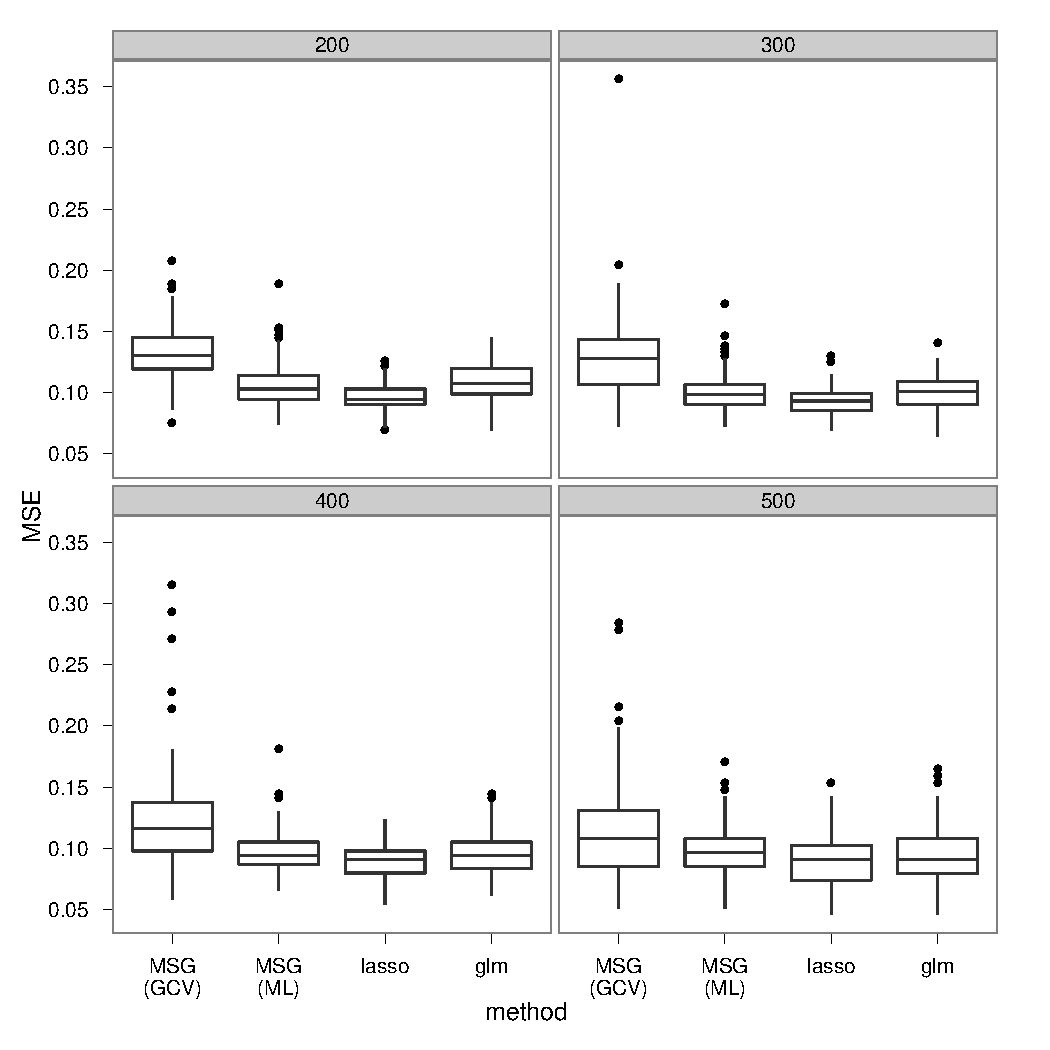
\includegraphics[width=6in]{gds/figs/mp-mse.pdf} \\
\caption{Boxpot of MSE per model for the MP free vote data set at varying sample sizes. The MSE for the lasso was significantly different (and smaller) than all of the other models by a pairwise Wilcoxon signed rank test (at the 0.01 level).}
\label{gds-mps-mse}
% generated by duchon/mps/analyse-mps.R
\end{figure}

\begin{figure}
\centering
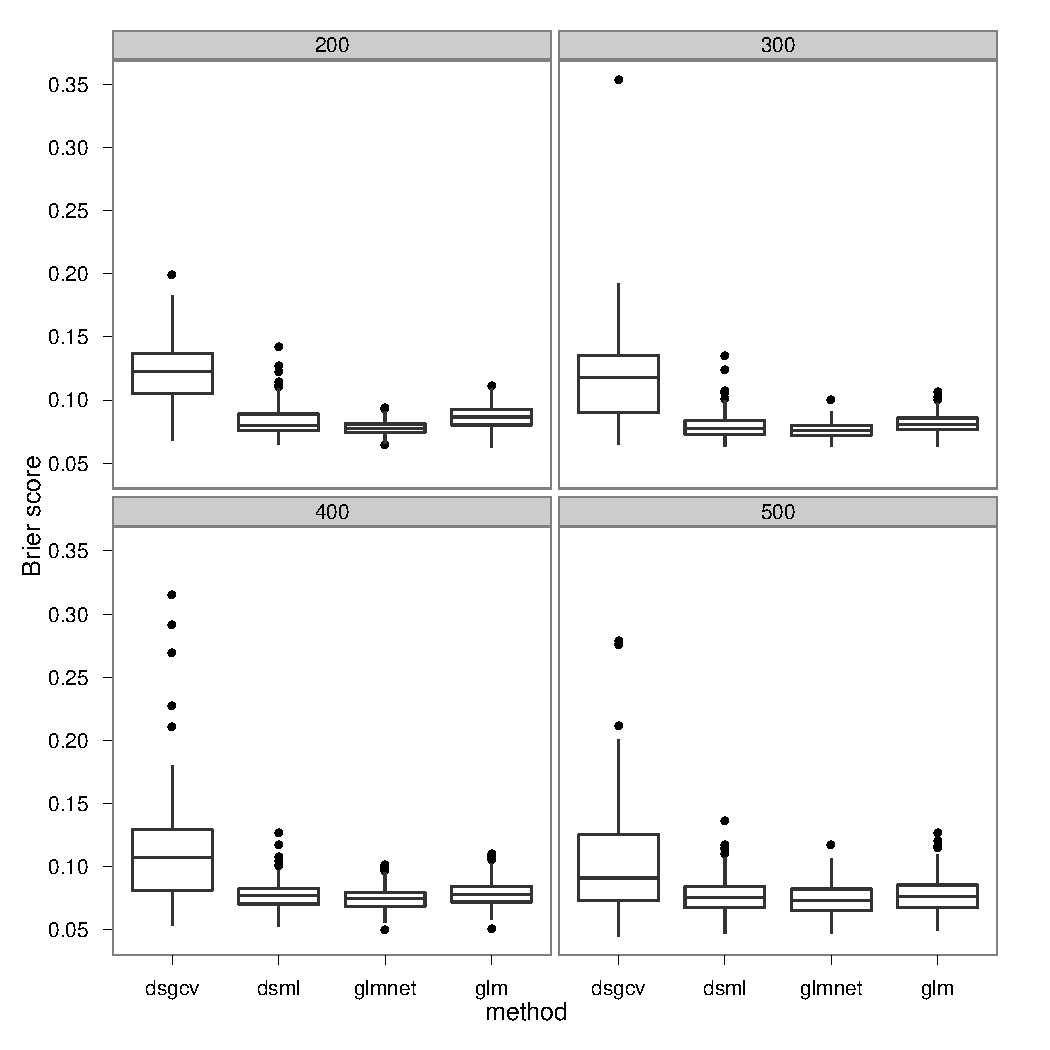
\includegraphics[width=6in]{gds/figs/mp-brier.pdf} \\
\caption{Boxplot of Brier score per model for the MP free vote data set at varying sample sizes. The Brier score for the lasso was significantly different (and smaller) than all of the other models by a pairwise Wilcoxon signed rank test (at the 0.01 level).}
\label{gds-mps-brier}
% generated by duchon/mps/analyse-mps.R
\end{figure}

Figures \ref{gds-mps-mse} and \ref{gds-mps-brier} show boxplots of the MSE and Brier scores respectively at the sample sizes used. The picture painted by the results is unambiguous and consistent across sample sizes: the lasso out-performs other methods. Interestingly, using the $\text{ML}_P$ score rather than the GCV score for the MDS projection dimension yields both a lower median MSE and a smaller standard error. Looking at the plots of score against dimension per simulation (figure \ref{gds-mps-dimselect}), we can see that per simulation (the black lines) the GCV score appears to be much more volatile than the $\text{ML}_P$ criterion. The selected projection dimensions (red dots) are spread across the whole range, showing no clear preference for one over another. Smooths (blue lines, green confidence bands) through the full set of scores do not show that there is any particular, definite minima of the scores in dimension. Figure \ref{gds-mps-edf} shows histograms of the EDFs (\secref{GAMEDF}) for the GCV and $\text{ML}_P$ selected models at the varying sample sizes. These plots clearly show that the EDFs for GCV are bimodal (and become more so at higher sample sizes) and that $\text{ML}_P$ selects models with significantly lower EDFs.

\begin{figure}
\centering
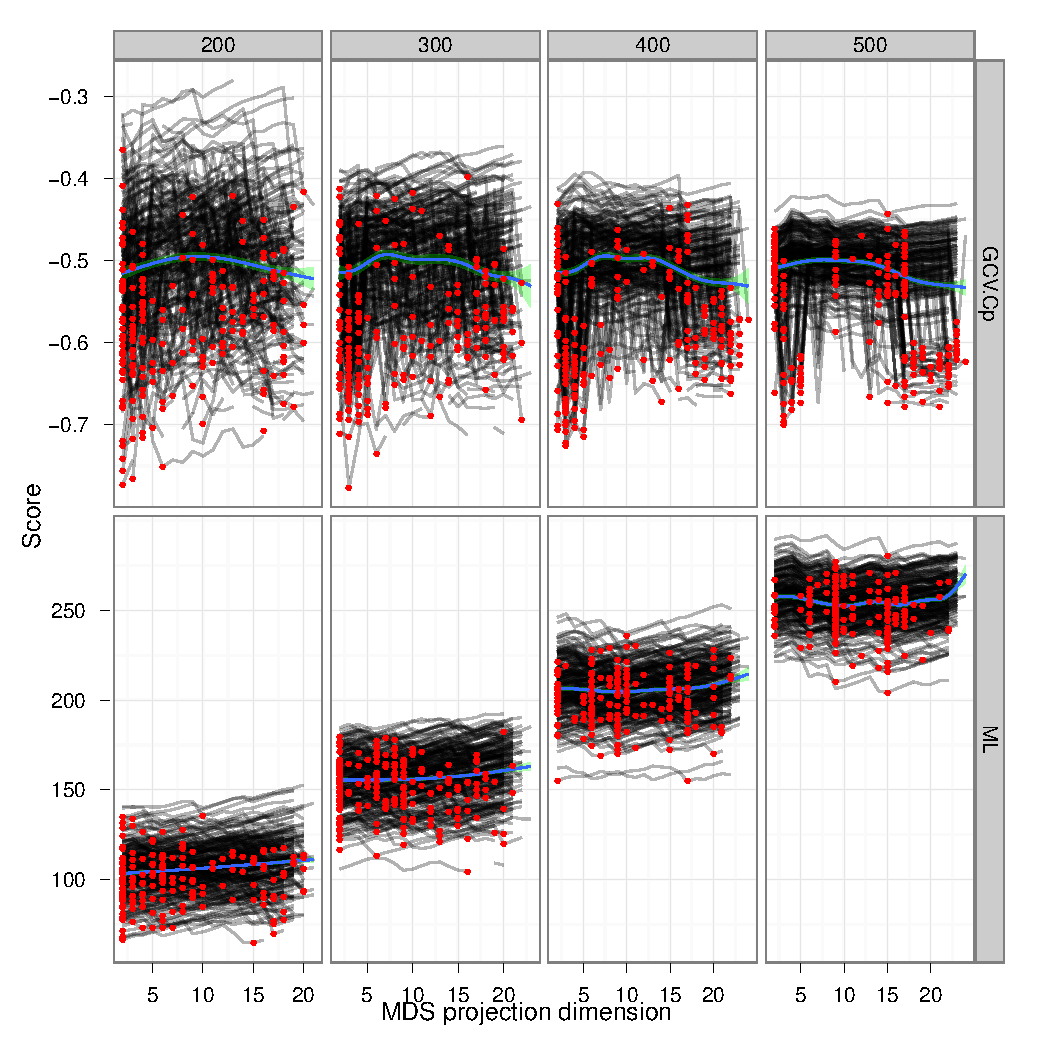
\includegraphics[width=6in]{gds/figs/mps-dimselect.pdf} \\
\caption{Plots of MDS projection dimension against score (GCV and $\text{ML}_P$) for the MP voting simulation per sample size. Each line represents one round of cross validation (some lines are broken due to convergence failure in the GAM), red dots indicate the selected projection dimensions (score minima) per simulation, blue lines are (thin plate regression spline) smooths through the full data set and the green bands are confidence bands.}
\label{gds-mps-dimselect}
% generated by duchon/mps/analyse-scoredim.R
\end{figure}

\begin{figure}
\centering
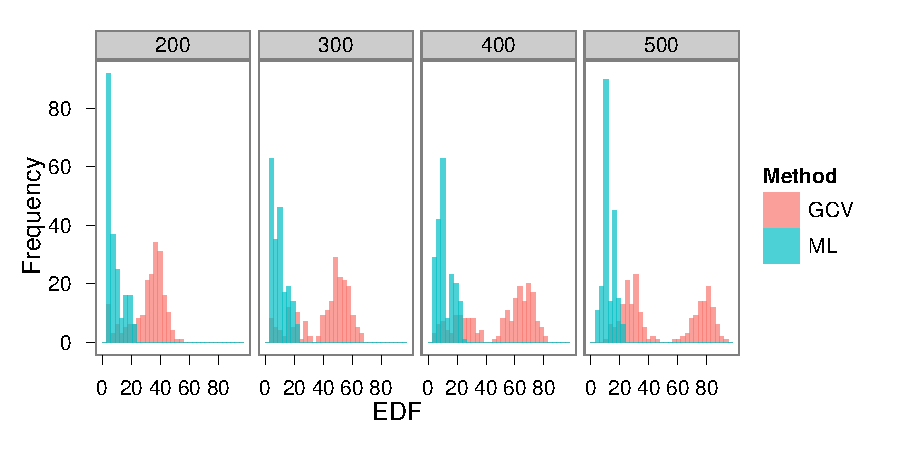
\includegraphics[width=6in]{gds/figs/mps-edf.pdf} \\
\caption{Histogram of EDFs of the selected models for the free vote simulation. When dimension selection is performed via GCV the EDFs are bimodal. In contrast the histogram of EDFs for the models selected by $\text{ML}_P$ shows a clear mode much lower than for GCV.}
\label{gds-mps-edf}
% generated by duchon/mps/analyse-edf.R
\end{figure}


\mdsds's performance in predicting MPs allegiance using the free vote data is disappointing. This poor performance may be due to there not being enough information in the distances to predict the party; since the data were ternary (votes were coded only $-1$, $0$ or $1$) there would be many distances that were similar. This theory is supported by looking at distance matrix for all MPs for the free votes, in that matrix there are only 63 unique values out of a possible $\binom{17}{3}=680$ (17 votes, with a ternary decision). Also worth noting is potential confounding between Labour MPs (which made up 429 out of the 676) and other ideologically similar parties (such as Plaid Cymru, SDLP and the Liberal Democrats (at that time)) which might cause potential problems when classifying. This, second, theory is less likely (given the performance of the lasso and GLM) but in combination with the first seems plausible. There is also something interesting happening in the differences between the GCV and $\text{ML}_P$ results.  GCV seems to prefer fitting models with higher EDFs than the $\text{ML}_P$, this may be an manifestation of the phenomena reported in \secref{intro-extending-gams}.

\subsubsection{Breast cancer microarrays}

Microarrays consist of small silicone or glass chips on which thousands of strands of RNA (which can be thought of as carrying instructions from DNA about how to create proteins) are stuck. These strands are known as \textit{targets} or \textit{probes}. When RNA from the sample comes into contact with that on the chip \textit{hybridisation} occurs (hydrogen bonds form between matching pairs). The targets are have a fluorescent die applied to them before hybridisation and can be scanned afterward to quantify the number of strands from the sample which have attached themselves to the chip, this is known as the \textit{expression level}.

\citeb[pp. 7-9]{ernstbook} describe a data set where both microarray and non-genetic data were collected on 62 patients with breast cancer. Rather than using RNA on the microarray, the experiment used DNA from cancer tissue and measured the differences between the genomic DNA of patients with breast cancer as compared to controls; the theory predicting that cancer causes loss of genetic material or additonal copies of genes to be obtained. The microarray contains expression data on 59 genes. Among the non-genetic data collected was the Nottingham Prognostic Index (NPI) (\cite{Haybittle1982} and \cite{Todd1987}), thought to be a good general measure of prognosis for patients with primary breast cancer (ie. cancer that has not spread beyond the breast). The NPI combines three pieces of information in a simple equation
\begin{equation}
\text{NPI} = 0.2(\text{size of index lesion in cm}) + \text{number of lymph nodes} + \text{tumour grade}.
\end{equation}
Further information can be found in the references above; it suffices to say that high values of NPI are bad, identifying those patients with very poor prognoses.

Rather than attempt to predict survival based on microarray data while controlling for other factors (as was the case in \cite[pp. 240-245]{ernstbook}), here the NPI is to be predicted based on the microarray data. This is not an unreasonable proposal since if one believes that there is some genetic mechanism behind breast cancer (or at least an individuals vulnerability/resistance to it) then the factors making up the NPI could be considered proxies for susceptibility. 

\citeb{spang2002} propose that rather that considering a large number individual genes, combinations are used. \citeb{spang2002} use a singular value decomposition of the microarray data to perform dimension reduction. The quantities resulting being referred to as ``super-genes''. In a similar way, using distances between patients and then taking the MDS projection, we can consider ``eigen-genes''.

Section \ref{gds-gds-examples} noted that both errors and non-standardised columns in the data matrix can cause issues with MDS since those variables with the greatest degree of variation do not necessarily contain the most information. One can easily imagine the case in which a completely unrelated gene was measured with huge error and then made up a huge proportion of the first eigenvalue in the decomposition of the distance matrix, this would dominate the projection but contain no information about the prediction (see also \cite[pp. 220-221]{ernstbook}). To get around this problem, rather than use the Euclidean distance between patients, the \textit{Mahalanobis distance} (\cite{mahalanobis}) can be used.

The Mahalanobis distance is easily calculated in the following way. Let $\mathbf{x}_{i}$ be a single row from the microarray matrix, $\mathbf{X}$, so that $\mathbf{x}_{i}$ is the vector gene expressions for a single patient. Under the assumption that all of the subjects are drawn from the same multivariate distribution some mean and covariance matrix $\mathbf{\Sigma}$, the Mahalanobis distance $d^\text{M}_{ij}$, between subjects $i$ and $j$ is then defined as:
\begin{equation}
d^\text{M}_{ij} = (\mathbf{x}_{i} - \mathbf{x}_{j})^\text{T} \mathbf{\Sigma}^{-1} (\mathbf{x}_{i} - \mathbf{x}_{j}),
\end{equation}
where $\mathbf{\Sigma}^{-1}$ is replaced with the inverse of the sample covariance matrix of $\mathbf{X}$. The calculated distance takes into account that the data may be more variable in some directions than in others. Calculating the Mahalanobis distance for each pair of patients and putting this into a distance matrix, we can then obtain the MDS projection in the same way as we would with a set of within-area or Euclidean distances. \citeb{gentleman2005} suggest using the Mahalanobis distance in a microarray setting.

Of the 62 patients in the study, 45 had non-missing values for NPI and out of the 59 genes in the microarray, 27 did not have missing values. In order to keep the analysis simple the NPI measurements of 45 patients using distance from 27 genes (i.e. the non-missing data) was used. For the MDS projection a lower bound of 2 and an upper bound of 85\% of the variation in the (sample) distance matrix was used (this equated to 19 or 20 dimensions usually). A number of different \mdsds\ models were fitted, with various error distributions. Using standard checks (eg. \texttt{gam.check()} in \texttt{mgcv}, fitting to residuals etc) two were deemed most promising. Those were a model with normal errors and one using a quasi-likelihood (\cite{quasi}, \cite{wood2008}) with a square root link function and variance proportional to the square of the mean. For comparison the lasso was (again) used. The implementation of the lasso does not allow the use of quasi-likelihood, so the normal model for \mdsds\ is a fairer comparison. 

Since the sample size is rather small, it was not possible to reasonably split the data into training and validation sets as with the MP data. Instead, leave-one-out cross validation (LOOCV) (\secref{DEFN-LOOCV}) was used to assess the sensitivity of the models to changes in the data, as well as overall prediction. Table \ref{breast-cancer-cv-results} and figure \ref{breast-cancer-cv-plot} show the results. Both the table and plot show that although \mdsds\ has a slightly lower LOOCV score than the lasso across the board and that the variability in the models is about the same. Performing a paired Wilcoxon (paired) signed rank test showed that each of the \mdsds\ models were not different from the lasso.

\begin{table}  
\begin{centering}
\begin{tabular}{cccc}
    Model & Mean & Median & Standard error \\ 
    \hline
lasso                 & 1.67  & 1.021  & 1.837 \\
\mdsds\ (GCV) - normal & 1.41  & 0.695  & 1.759 \\
\mdsds\ (ML) - normal  & 1.426 & 0.629  & 1.873 \\
\mdsds\ (GCV) - quasi  & 1.427 & 0.654  & 1.739 \\
\mdsds\ (ML) - quasi   & 1.419 & 0.575  & 1.857 \\
  \end{tabular}
\caption{Summary of the results for the breast cancer cross validation. Summary statistics are over 45 rounds of cross validation.}
\end{centering}
% generated by duchon/breast/analyse-cv.R
\label{breast-cancer-cv-results}
\end{table}

\begin{figure}
\centering
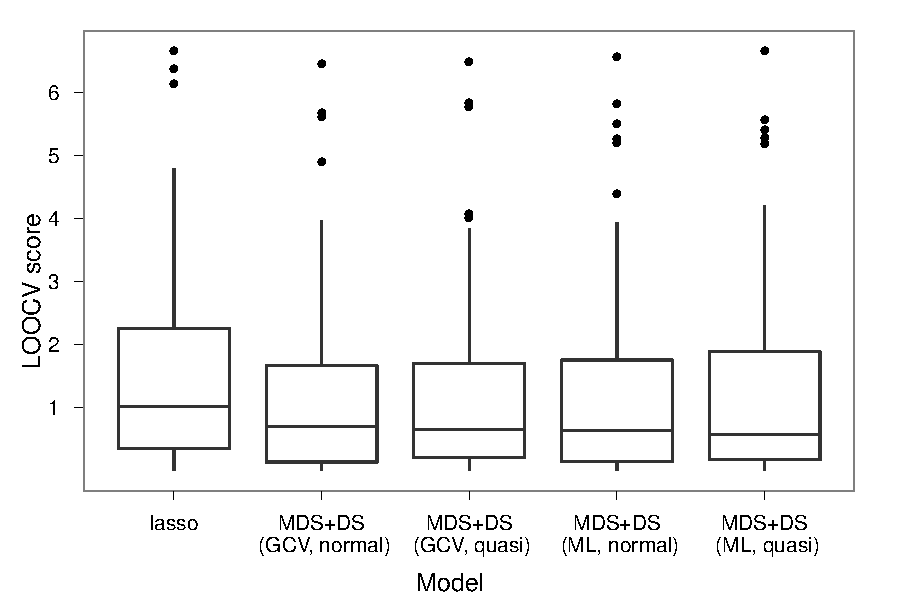
\includegraphics[width=6in]{gds/figs/breastcancer-cv-plot.pdf} \\
\caption{Boxplots of the LOOCV score per model for the breast cancer cross validation. A Wilcoxon (paired) signed rank test did not show that there was a significant difference between the \mdsds\ models and the lasso (in fact $p>0.5$ in every case).}
\label{breast-cancer-cv-plot}
% generated by duchon/breast/analyse-cv-plot.R
\end{figure}

Figure \ref{breastcancer-dimselect} shows the plots of MDS projection dimension against score, each line represents one round of cross validation (some lines are broken due to convergence failure in the fitting routine), red dots indicate minima in the score per simulation (the selected dimension) and the blue lines are (thin plate regression spline) smooths through the full data set to give a general idea of what is going on (with green confidence bands). Both error distributions show a similar relationship between dimension and score.

The GCV score appears to have a minima somewhere between 5 and 11 dimensions, which is fairly well defined given the size of the data set.  $\text{ML}_P$, on the other hand, appears to select high dimensional solutions (almost all models were either 19 or 20 dimensions). Upon first inspection one might think that the optima was at 19 or 20 and that this was a true minima. Further analysis shows that this is not the case. Increasing from 85\% of the variation to 95\% and 99\% of the variation only pushes the $\text{ML}_P$ ``minima'' to higher dimensions. This behaviour may indicate that the penalization used for $\text{ML}_P$ is not strong enough in the generalized distance case. Comparison of penalized versus unpenalized scores shows that the penalty is having some effect (and local minima are introduced) but this is not enough to introduce a global minima that is not at the highest dimension.

\begin{figure}
\centering
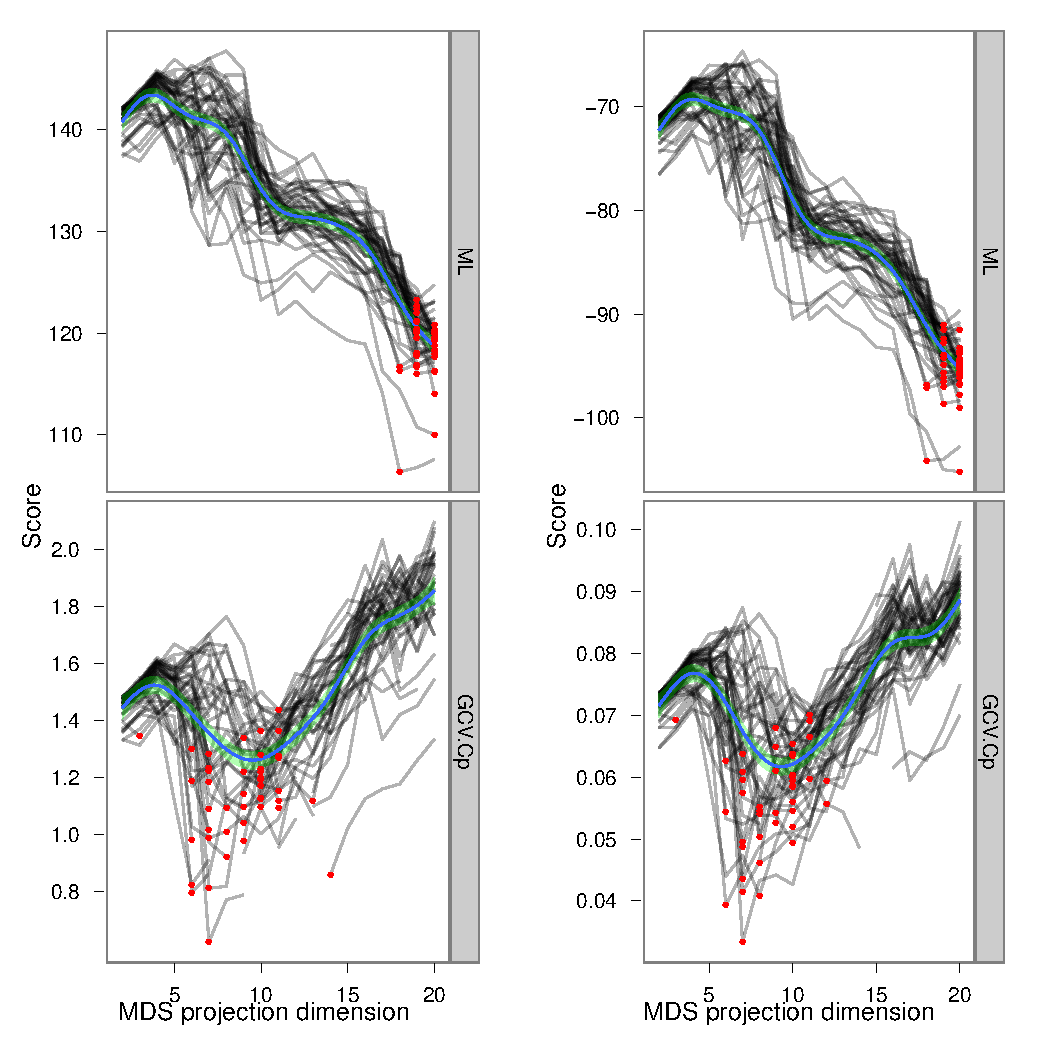
\includegraphics[width=6in]{gds/figs/breastcancer-dimselect.pdf} \\
\caption{Plots of MDS projection dimension against score (GCV and $\text{ML}_P$) for both normal (left) and quasi-likelihood (right) models for the breast cancer microarray LOOCV. Each line represents one round of cross validation (some lines are broken due to convergence failure in the GAM), red dots indicate the selected projection dimensions (score minima) per simulation, blue lines are (thin plate regression spline) smooths through the full data set and the green bands are confidence bands.}
\label{breastcancer-dimselect}
% generated by duchon/breast/analyse-dimselect.R
\end{figure}

This analysis shows that although \mdsds\ can be used for generalized distance smoothing in a microarray setting, it is far from conclusive that the methods out performs the lasso. Choice of the metric used to calculate the distances has a large influence on the results (preliminary results using Euclidean distance were much worse in terms of the results from the LOOCV). It would be interesting to investigate the behaviour of the $\text{ML}_P$ score further on larger data sets to see why such high dimensional models are chosen. The study here is rather small and specialized, therefore it is hard to draw a conclusion about how \mdsds\ will perform in other situations, although its performance here against the lasso (technique that has been in development for considerably longer) is encouraging. The final analysis again looks at microarray data in an attempt to further investigate the utility of \mdsds\ for microarray data.

\subsubsection{Leukemia microarrays}

\citeb{yeoh2002} investigate expression data from 327 patients with acute lymphoblastic leukaemia (ALL), collected on 12626 genes. The original purpose of the study was attempting to classify patients into one of ten prognostically important ALL subtypes (since treatment is dependent on subtype), based on looking at the expression data. \citeb{yeoh2002} used heirarchical clustering to find groupings of genes in the data and then found those groups corresponded to particular ALL subtypes. Genes were ranked per subtype according a $\chi^2$ statistic (based on the expected value per cluster) to find the most relevant genes for each subtype. The ``true'' diagnoses had been found by other methods. More information on the study may be found at \url{http://www.stjuderesearch.org/data/ALL1}.

To simplify the analysis here, a binary response was used (of a particular subtype versus not that subtype, as with the MPs' parties above). In all four simulations settings were used, varying the model and data. Two simulations used the whether the patient had the TEL-AML1 subtype as the response (TEL-AML1 was the largest group, with 79 patients) and two simulations used T-ALL (43 patients were diagnosed with T-ALL). For each subtype two different simulations were run: ($i$) the 40 genes selected by $\chi^2$ as the best indicators of that subtype were used as the data and ($ii$) those 40 genes chosen by $\chi^2$ with an additional 100 genes chosen at random (but kept the same over realisations). 

The two scenarios show the difference between an idealised situation where the best predictors have already been found versus a more realistic situation in which there is a lot of noise from non-relevant genes. In each of the simulations 100 realisations were generated and in each of these 215 patients were selected as samples and models fit using their data (as was the case in \cite{yeoh2002}). Models were then used to predict the classes of the remaining 112 patients. Brier scores and MSEs were recorded. Models using both ML and GCV dimension selection were used and as above, the lasso was used for comparison using the same settings as in the MP example. 

Unfortunately the results are not encouraging at all. For both the T-ALL and TEL-AML1 data, both with and without the additional confounding genes, the lasso outperformed \mdsds\ by a large margin. Boxplots of MSE and Brier scores are shown in figure \ref{leuk-sim-boxplot}. The boxplots show clearly that the lasso is much better suited to this type of problem.

\begin{sidewaysfigure}
\centering
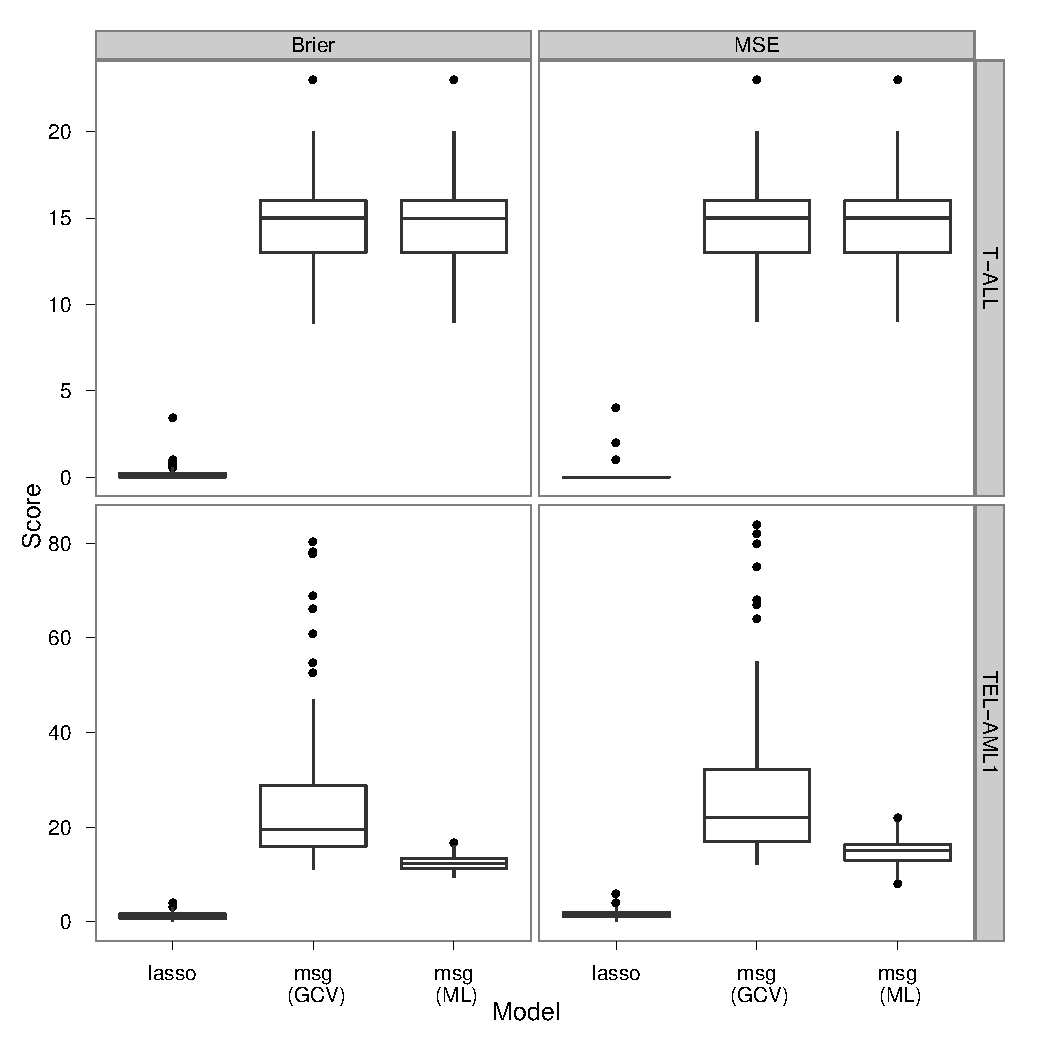
\includegraphics[width=4in]{gds/figs/sim-msebrier.pdf} 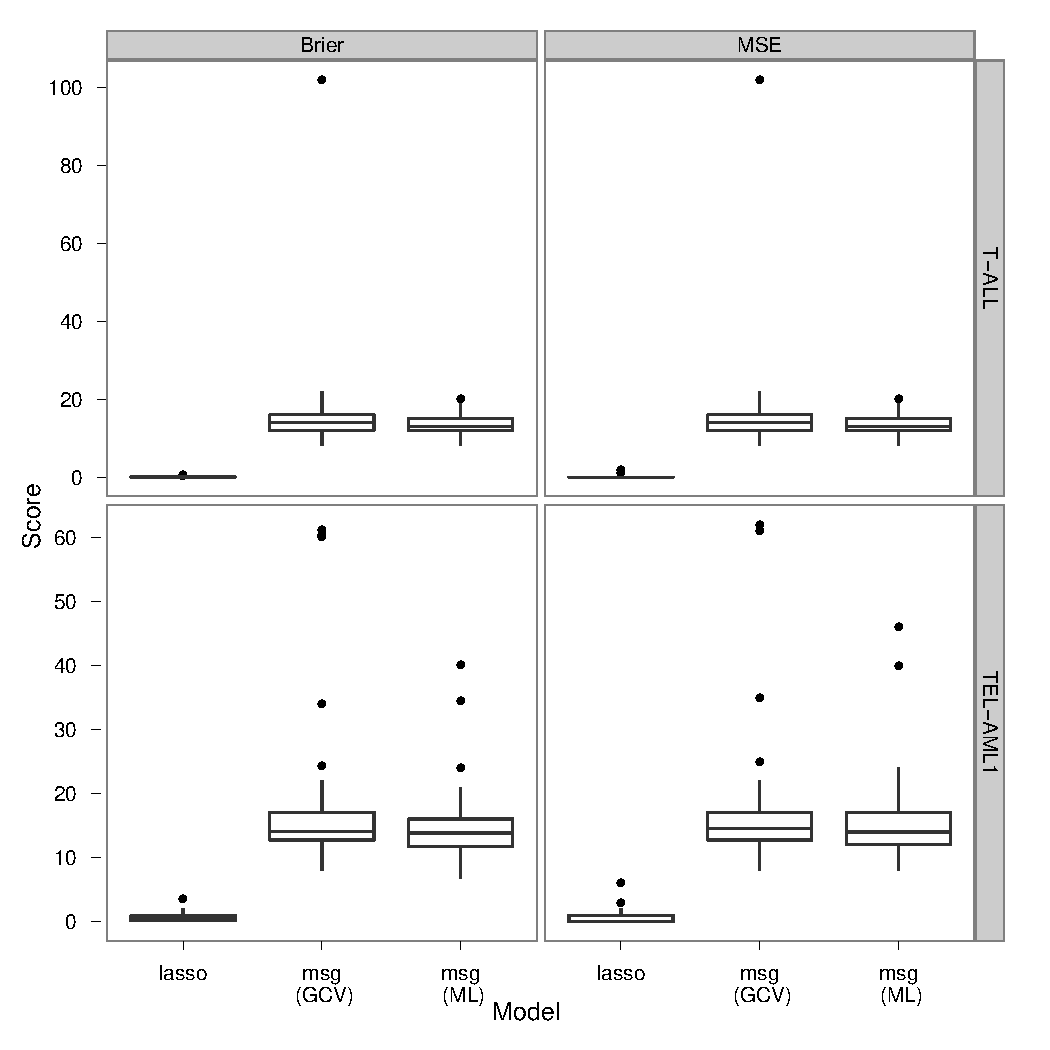
\includegraphics[width=4in]{gds/figs/confsim-msebrier.pdf} \\
\caption{Boxplot of Brier and MSE scores (columns) for the T-ALL and TEL-AML1 data (rows) when left: the 40 genes selected by $\chi^2$ were used and right: 100 extra genes were used for each of the models fit (lasso, \mdsds\ with $\text{ML}_P$ and \mdsds\ with GCV dimension selection. The lasso vastly outperforms \mdsds.}
\label{leuk-sim-boxplot}
% generated by duchon/leuk/analyse-sim.R
\end{sidewaysfigure}

\begin{table}  
\begin{centering}
\begin{tabular}{c || ccc | ccc}
    &  & MSE &  &  & Brier & \\ 
Model & Mean & Median & Standard error & Mean & Median & Standard error \\
\hline
\textit{T-ALL} & & & & & & \\
lasso &  0.26 & 0 & 0.06 & 0.19 & 0.02 & 0.04 \\
MSG (GCV) & 14.81 & 15 & 0.25 & 14.8 & 15 & 0.25 \\
MSG ($\text{ML}_P$) &  14.79 & 15 & 0.26 & 14.74 & 14.99 & 0.26 \\
\textit{TEL-AML1}  & & &  & & & \\
lasso &  1.59 & 1.5 & 0.12 & 1.29 & 1.19 & 0.08 \\
MSG (GCV) & 31.44 & 20.5 & 2.3 & 29.11 & 18.29 & 2.24 \\
MSG ($\text{ML}_P$) &  14.59 & 15 & 0.28 & 12.97 & 12.98 & 0.18 \\
  \end{tabular}
\caption{Summary of the results for the leukaemia simulation when the 40 genes selected by \citeb{yeoh2002} using $\chi^2$ were used. Note the huge difference between the lasso and \mdsds\ results.}
\end{centering}
% generated by phd-smoothing/duchon/leuk/analyse-sim.R 
\label{leuk-sim}
\end{table}


\begin{table}  
\begin{centering}
\begin{tabular}{c || ccc | ccc}
    &  & MSE &  &  & Brier & \\ 
    Model & Mean & Median & Standard error & Mean & Median & Standard error \\
    \hline
\textit{T-ALL}  & & & & & & \\
lasso &  0.14 & 0 & 0.06 & 0.1 & 0.02 & 0.02 \\
MSG (GCV) & 15.14 & 14 & 0.96 & 15.13 & 14 & 0.96 \\
MSG ($\text{ML}_P$) &  13.75 & 13 & 0.36 & 13.74 & 13 & 0.36 \\
\textit{TEL-AML1}  & & & & & & \\
lasso &  0.94 & 1 & 0.11 & 0.63 & 0.45 & 0.06 \\
MSG (GCV) & 16.1 & 14.5 & 0.89 & 16.01 & 14.09 & 0.88 \\
MSG ($\text{ML}_P$) &  14.81 & 14 & 0.54 & 14.31 & 13.84 & 0.48 \\
  \end{tabular}
\caption{Summary of the results for the leukaemia simulation when 100 extra confounding genes were added to the 40 selected using $\chi^2$. The lasso performs extremely well, even with 100 confounding genes.}
\end{centering}
% generated by phd-smoothing/duchon/leuk/analyse-confsim.R 
\label{leuk-confsim}
\end{table}

Tables \ref{leuk-sim} and \ref{leuk-confsim} show that \mdsds\ does not even begin to approach the predictive power of the lasso on this data set. One might expect that the lasso would perform well on the dataset consisting of only the 40 genes selected by \citeb{yeoh2002} (and indeed that \mdsds\ would perform better), however it is extremely impressive that the lasso has such a low MSE and Brier score for the data with the confounding genes. This may, however, give some insights into why \mdsds\ has such poor performance. 

\begin{sidewaysfigure}
\centering
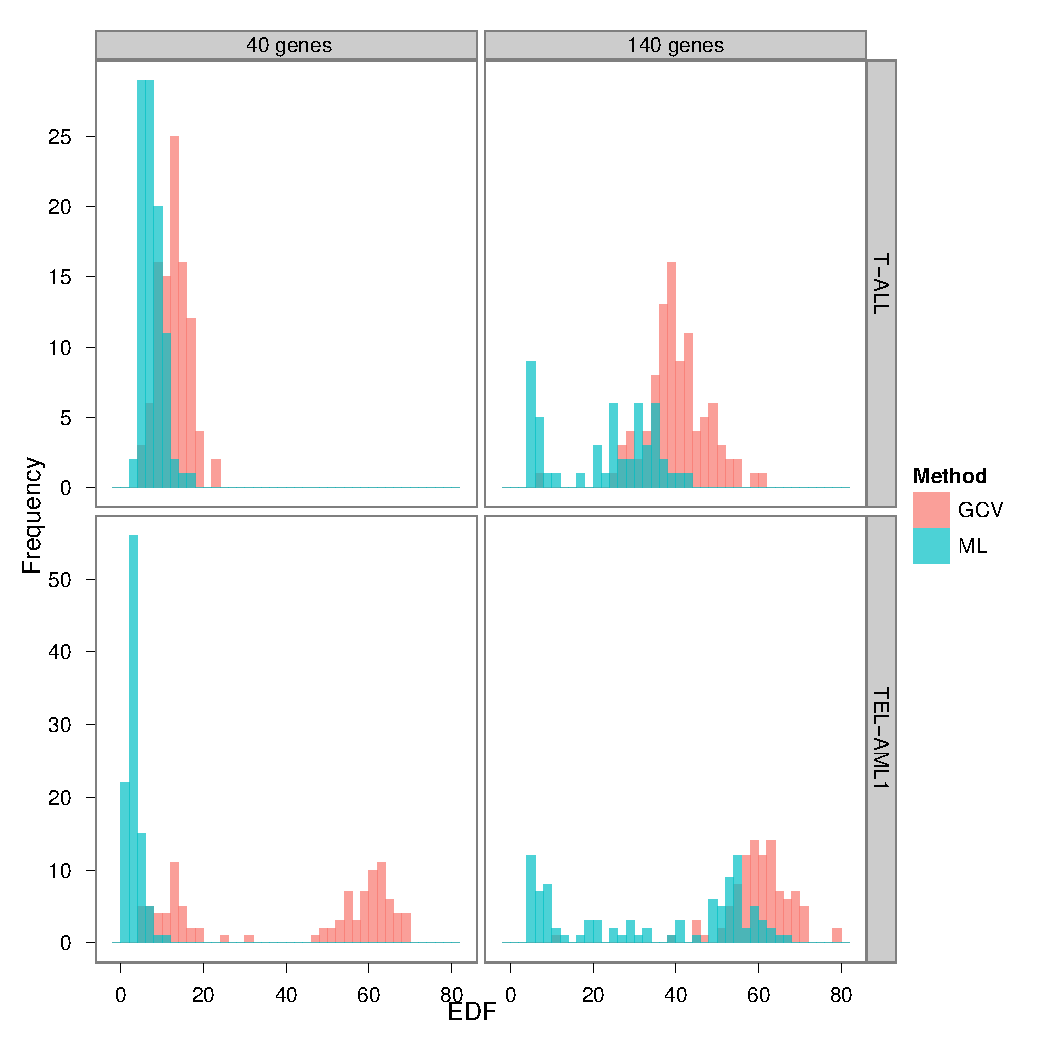
\includegraphics[width=4in]{gds/figs/leuk-edf.pdf} 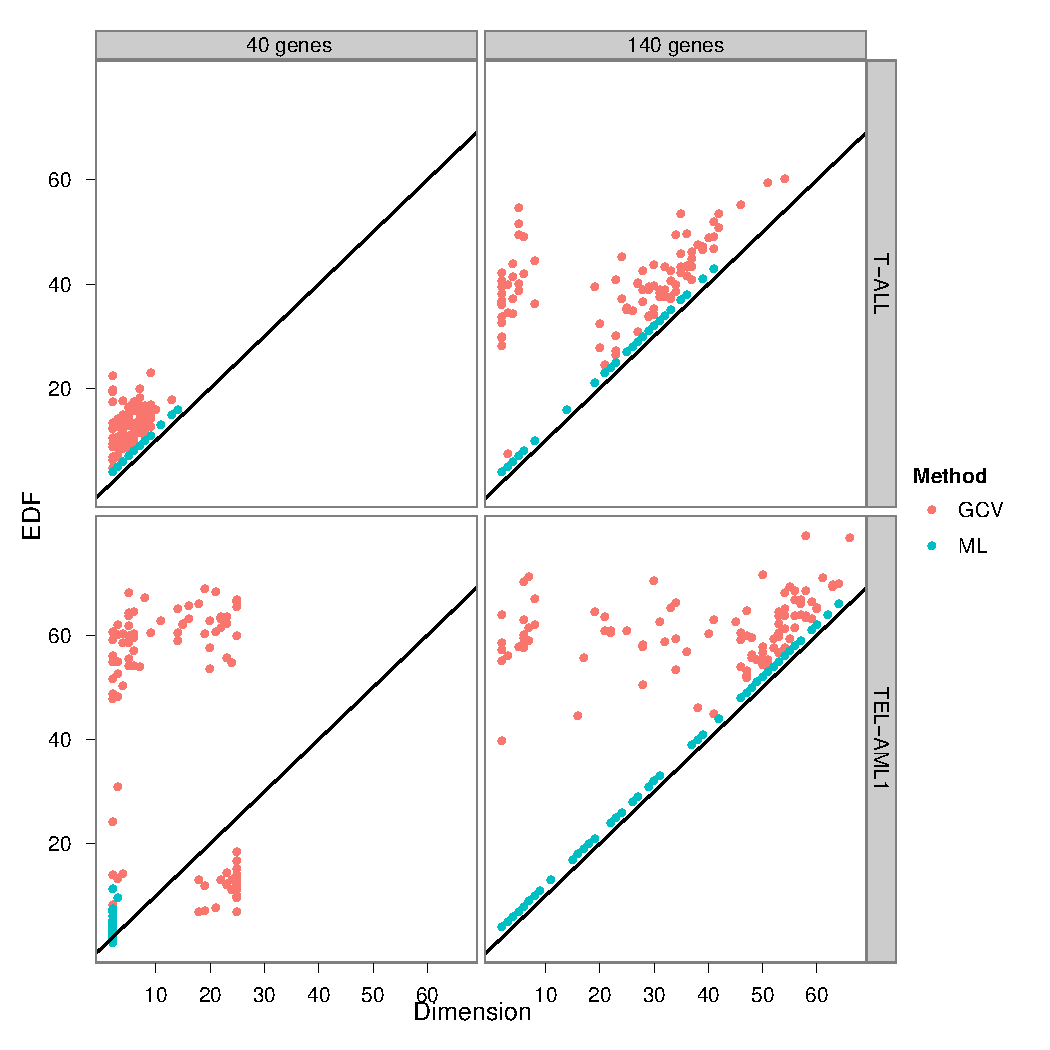
\includegraphics[width=4in]{gds/figs/leuk-dim-edf.pdf} \\
\caption{EDF and MDS projection dimension selection investigation for the leukaemia data. Left: histogram of EDFs of the models selected by GCV (red) and $\text{ML}_P$ (blue). Right: plot of EDF against selected MDS projection dimension (with the same colour coding), lines of $x=y$ are included to aid comparison. The histograms on the left of the figure are the marginals of the plots on the right.}
\label{leuk-edf}
% generated by duchon/leuk/analyse-edf.R
\end{sidewaysfigure}

Concentrating on the \mdsds\ results, some information can be gleaned from these results, aside from the fact that the performance of \mdsds\  is not as good as that of the lasso. The left panel of figure \ref{leuk-edf} shows histograms of the EDFs of the models selected by GCV and ML. Similarly to the models fit to the MP voting data, above, it appears that $\text{ML}_P$ selects models that in general have lower EDFs than those selected by GCV. However, this time there is bimodality in the $\text{ML}_P$ histograms (or at least, no clear single mode). 

Generally GCV selected much more complex models than $\text{ML}_P$, in all but one simulation setting (40 genes with TEL-AML1) $\text{ML}_P$ selected models that had EDFs only slightly bigger than the dimension. This corresponds to $\text{ML}_P$ fitting (hyper)planes to the data. The results for $\text{ML}_P$ are in general slightly better than for GCV selection (tables \ref{leuk-sim} and \ref{leuk-confsim}), except for the 40 genes case for TEL-AML1 where the $\text{ML}_P$ results are significantly better. These results may well be an manifestation of the behaviour described in \secref{intro-extending-gams}: that GCV gives much more variable smooths. 

The performance of $\text{ML}_P$, combined with the EDF/dimension selection behaviour indicates that perhaps the assumption of a smooth response is not appropriate. Given the performance of the lasso, this seems likely. It is rather difficult to test for this graphically in such high dimensions, but the EDFs do seem to indicate that this is the case.

Another potential source of poor performance is the metric used to find the distances. Although the Mahalanobis distance may be an obvious choice, there may be other measures that provide better results.


\subsection{Conclusion}

Although in the spatial setting \mdsds\ appears to perform very well, when used as a dimension reduction technique it fails. Between examples the results are quite variable, with a lack of conclusive behaviour. Within each example the results are also variable and it is difficult to draw a solid conclusions. It would however appear that the metric used to calculate the distances plays a key role in the performance of \mdsds, as one would expect. Drawing an analogy to the finite area smoothing case, if the Euclidean metric is used with MDS then the projected space is exactly the same as before the projection (up to scaling and rotation) but when the within-area distances are used then a much more reasonable set of points are generated (from a smoothing perspective). It is not unreasonable to believe that a similar situation is the case for the generalized distance case.

Another factor may be that in the examples above, in each case the response may not have been non-linear enough to warrant the use of the smoothers used. This is partially captured in the plots of the EDFs against selected dimension (figure \ref{leuk-edf}) and in the good performance of the lasso in all situations. There was a hint in the leukaemia data that the results from GCV were more variable than those of ML (as discussed in \secref{intro-extending-gams}), however this does not appear to manifest itself as a general problem with \mdsds\ since, looking at figure \ref{mps-edf-dim} the EDF-dimension relationship exhibits the opposite relationship -- $\text{ML}_P$ is much more variable.

\begin{figure}
\centering
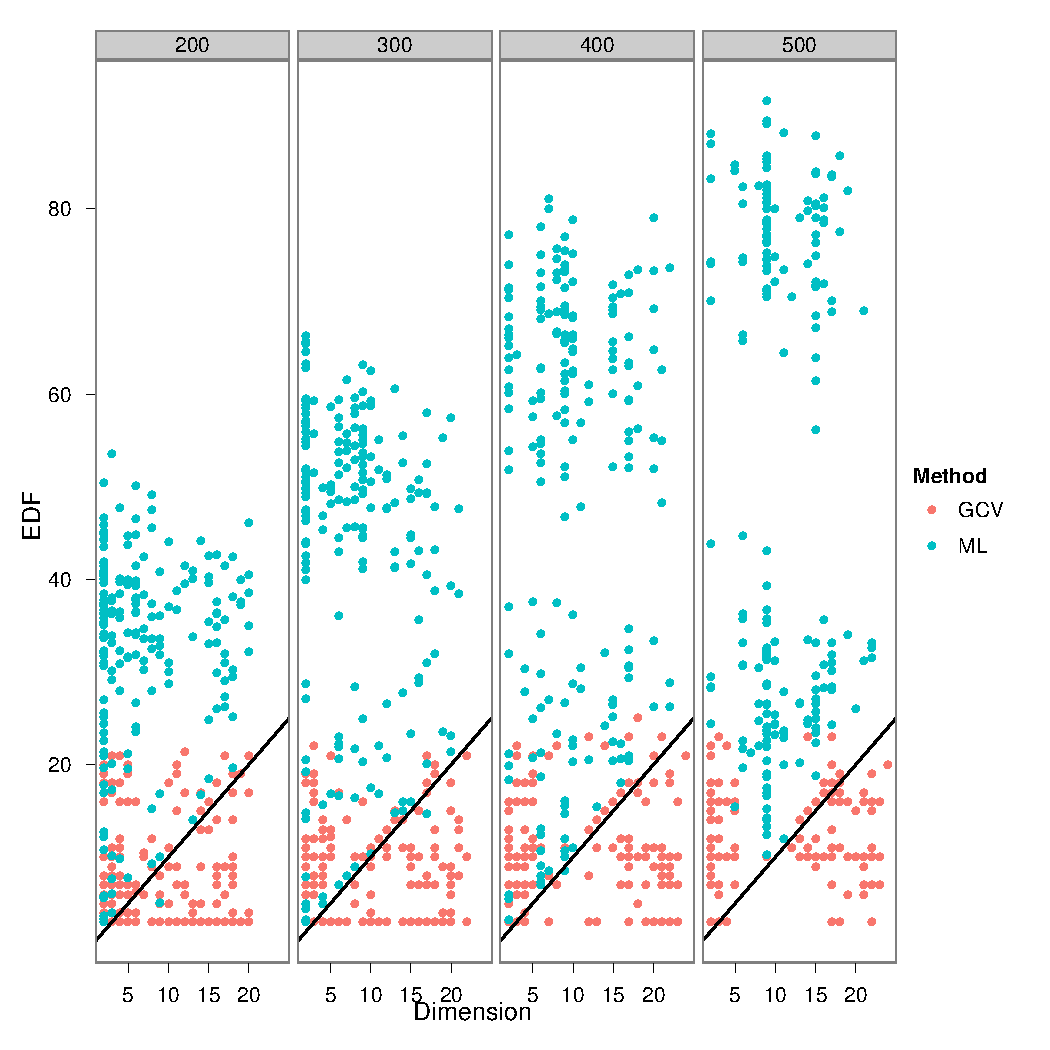
\includegraphics[width=6in]{gds/figs/mps-dim-edf.pdf} \\
\caption{Relationship between EDF and selected dimension for the MP voting data set. Diagonal line shows where EDF would equal dimension. In this situation $\text{ML}_P$ is much more variable.}
\label{mps-edf-dim}
% generated by duchon/mp/analyse-edf-dim.R
\end{figure}

An additional consideration in the poor performance in the MP voting data and the leukaemia data is that there response was binary, which makes model checking rather difficult. For the breast cancer data the combination index may also have complicated matters. Finding data which have a continuous response might yield interesting results (it is possible that in the breast cancer data the sample size was a key issue, although \mdsds\ did marginally outperform the lasso).

In all of the example data sets, the issue of choosing an appropriate distance measure is vital. Several other options were used before settling on those which are investigated here. Results varied according to the measure that was used. With gene expression data there is an obvious conflict between the MDS methodology and what one would like to do to make predictions as accurate as possible. As discussed above, different genes will express at different levels and there may be measurement errors in the data. Using Mahalanobis distance allows the procedure to account for the variability in the data, however it does not account for outliers. Outliers can cause problems with MDS, changing the resulting point configuration in an extreme way.

Although \mdsds\ does not perform better than the lasso in the dimension reduction-type tasks shown here, there is certainly promise in the method. If it is possible to control better for the presence of outliers and for differing variances between columns via the distance measure used or a different metric, the method could become very useful. Finally, the model has a strong motivation for biological studies, since there is evidence that those who are genetically similar have a greater propensity to contract certain conditions (one only needs to think of hereditary conditions to see this). Having some way of relating the genetic distances between patients to the conditions that they present seems like a logical and useful development, provided that a useful measure of that distance can be found.
